\documentclass{sigplanconf}

\usepackage{amssymb}
%\usepackage{amsthm}
\usepackage{balance}
%\usepackage{breakurl}             % Not needed if you use pdflatex only.
\usepackage{color}
\usepackage{epsfig}
%\usepackage{esvect}
\usepackage{listings}
\usepackage{mathpartir}
\usepackage{MnSymbol}
\usepackage{multirow}
\usepackage{paralist}
\usepackage{rotating}
\usepackage{url}

\setlength{\parskip}{0cm}
%\setlength{\parindent}{1em}

\definecolor{mylightgray}{RGB}{220,220,220}
\definecolor{mygray}{RGB}{128,128,128}
\definecolor{mydarkgray}{RGB}{96,96,96}

\newcommand{\term}[1]{\emph{#1}}
\newcommand{\subterm}[2]{\emph{#2}}

\DeclareRobustCommand{\Cpp}{C\texttt{++}}
\DeclareRobustCommand{\code}[1]{{\lstinline[breaklines=false,escapechar=@]{#1}}}
\DeclareRobustCommand{\codebr}[1]{{\lstinline[breaklines=true]{#1}}}
\DeclareRobustCommand{\codehaskell}[1]{{\lstinline[breaklines=false,language=Haskell]{#1}}}
\DeclareRobustCommand{\codeocaml}[1]{{\lstinline[breaklines=false,language=Caml]{#1}}}
\DeclareRobustCommand{\concept}[1]{{\small\textsc{#1}}}

\newcommand{\exclude}[1]{}
\newcommand{\halfline}{\vspace{-1.5ex}}

\lstdefinestyle{C++}{language=C++,%
showstringspaces=false,
  columns=fullflexible,
  escapechar=@,
  basicstyle=\sffamily,
%  commentstyle=\rmfamily\itshape,
  commentstyle=\color{mygray},   % gray comments
  stringstyle=\color{mydarkgray}\rmfamily\itshape, % string literals in italics
  aboveskip=\medskipamount, % the space above displayed listings (\medskipamount)
  belowskip=\medskipamount, % the space below displayed listings (\medskipamount)
  lineskip=-1pt,            % additional space between lines in listings (0pt)
  moredelim=**[is][\color{white}]{~}{~},
  morekeywords={axiom,concept,constexpr,decltype,noexcept,nullptr,requires,static_assert},
  literate={[<]}{{\textless}}1      {[>]}{{\textgreater}}1 %
           {[<<]}{{$\ll$ }}2        {[>>]}{{$\gg$ }}2 %
           {*}{{$*$}}1 % Without this, star (*) is rendered in Type 3 font
           %{_}{{\textunderscore}}1 %
           {<}{{$\langle$}}1        {>}{{$\rangle$}}1 %
           {<=}{{$\leq$}}1          {>=}{{$\geq$}}1 %
           {==}{{$==$}}2            {!=}{{$\neq$}}1 %
           {=>}{{$\Rightarrow\;$}}1 {->}{{$\rightarrow{}$}}1 %
           {...}{{$\ldots$}}3
           {<:}{{$\subtype{}\ $}}1  {<-}{{$\leftarrow$}}1 %
           {s1;}{{$s_1$;}}3 {s2;}{{$s_2$;}}3 {s3;}{{$s_3$;}}3 {s4;}{{$s_4$;}}3 {s5;}{{$s_5$;}}3 {s6;}{{$s_6$;}}3 {s7;}{{$s_7$;}}3 {sn;}{{$s_n$;}}3 {si;}{{$s_i$;}}3%
           {P1}{{$P_1$}}2 {P2}{{$P_2$}}2 {P3}{{$P_3$}}2 {P4}{{$P_4$}}2 {P5}{{$P_5$}}2 {P6}{{$P_6$}}2 {P7}{{$P_7$}}2 {Pn}{{$P_n$}}2 {Pi}{{$P_i$}}2%
           {D1}{{$D_1$}}2 {D2}{{$D_2$}}2 {D3}{{$D_3$}}2 {D4}{{$D_4$}}2 {D5}{{$D_5$}}2 {D6}{{$D_6$}}2 {D7}{{$D_7$}}2 {Dn}{{$D_n$}}2 {Di}{{$D_i$}}2%
           {T1}{{$T_1$}}2 {T2}{{$T_2$}}2 {T3}{{$T_3$}}2 {T4}{{$T_4$}}2 {T5}{{$T_5$}}2 {T6}{{$T_6$}}2 {T7}{{$T_7$}}2 {Tn}{{$T_n$}}2 {Ti}{{$T_i$}}2 {Tm}{{$T_m$}}2%
           {e1}{{$e_1$}}2 {e2}{{$e_2$}}2 {e3}{{$e_3$}}2 {e4}{{$e_4$}}2%
           {E1}{{$E_1$}}2 {E2}{{$E_2$}}2 {E3}{{$E_3$}}2 {E4}{{$E_4$}}2%
           {_1}{{$_1$}}1  {_2}{{$_2$}}1  {_3}{{$_3$}}1  {_4}{{$_4$}}1  {_ii}{{$_i$}}1  {_nn}{{$_n$}}1  {_N}{{$_N$}}1%
           {[_1]}{{\_1}}2  {[_2]}{{\_2}}2 %
           {m_e1}{{$m\_e_1$}}4 {m_e2}{{$m\_e_2$}}4 {m_e3}{{$m\_e_3$}}4 {m_e4}{{$m\_e_4$}}4%
           {aa}{{$a$}}1 {bb}{{$b$}}1 {Cc}{{$c$}}1 {Dd}{{$d$}}1 {ff}{{$f$}}1 {mm}{{$m$}}1%
           {Ss}{{$s$}}1 {Tt}{{$t$}}1 {vv}{{$v$}}1 {xx}{{$x$}}1 {yy}{{$y$}}1 {zz}{{$z$}}1%
           {Divide}{{Divide}}6 {Either}{Either}6 %
           {Times}{{Times}}5 %
           {Match}{{\emph{Match}}}5 %
           {Case}{{\emph{Case}}}4 %
           {Qua}{{\emph{Qua}}}3 %
           {When}{{\emph{When}}}4 %
           {Otherwise}{{\emph{Otherwise}}}9 %
           {EndMatch}{{\emph{EndMatch}}}8 %
           {CM}{{\emph{CM}}}2 {KS}{{\emph{KS}}}2 {KV}{{\emph{KV}}}2 %
           {EuclideanDomain}{\concept{EuclideanDomain}}{15}  %
           {LazyExpression}{\concept{LazyExpression}}{14}    %
           {Polymorphic}{\concept{Polymorphic}}{11}          %
           {CopyConstructible}{\concept{CopyConstructible}}{17}%
           {MoveConstructible}{\concept{MoveConstructible}}{17}%
           {EqualityComparable}{\concept{EqualityComparable}}{18}%
           {Copyable}{\concept{Copyable}}8                   %
           {Convertible}{\concept{Convertible}}{11}          %
           {Integral}{\concept{Integral}}8                   %
           {SameType}{\concept{SameType}}8                   %
           {Pattern}{\concept{Pattern}}7                     %
           {Regular}{\concept{Regular}}7                     %
           {Field}{\concept{Field}}5                         %
}
\lstset{style=C++}

\lstdefinestyle{Haskell}{language=Haskell,%
  morekeywords={out,view,real},
  literate={=>}{{$\Rightarrow\;$}}1 {->}{{$\rightarrow{}$}}1 {<-}{{$\leftarrow$}}1 {\\}{{$\lambda$}}1,
  moredelim=**[is][\color{red}]{`}{`},
  moredelim=**[is][\color{white}]{~}{~}
}

\lstdefinestyle{GJ}{language=Java,
  moredelim=**[is][\color{red}]{`}{`},
  moredelim=**[is][\color{white}]{~}{~}
}
\lstdefinestyle{Eiffel}{language=Eiffel,%
  literate={->}{{$\rightarrow$}}1,
  moredelim=**[is][\color{red}]{`}{`},
  moredelim=**[is][\color{white}]{~}{~}
}
\lstdefinestyle{Csharp}{language=[Sharp]C,
  morekeywords={where,require,type},
  literate={->}{{$\rightarrow{}$}}1,
  moredelim=**[is][\color{red}]{`}{`},
  moredelim=**[is][\color{white}]{~}{~}
}

\lstdefinestyle{ML}{language=ML,%
  literate={->}{{$\rightarrow{}$}}1,
  moredelim=**[is][\color{red}]{`}{`},
  moredelim=**[is][\color{white}]{~}{~}
}

\lstdefinestyle{Caml}{language=[Objective]Caml,%
  morekeywords={when},
  literate={->}{{$\rightarrow{}$}}1,
  moredelim=**[is][\color{red}]{`}{`},
  moredelim=**[is][\color{white}]{~}{~}
}

\lstdefinelanguage{scala}{% 
   morekeywords={% 
                try, catch, throw, private, public, protected, import, package, implicit, final, package, trait, type, class, val, def, var, if, this, else, extends, with, while, new, abstract, object, requires, case, match, sealed,override},% 
   sensitive=t, % 
   morecomment=[s]{/*}{*/},morecomment=[l]{\//},% 
   escapeinside={/*\%}{*/},%
   rangeprefix= /*< ,rangesuffix= >*/,%
   morestring=[d]{"}% 
}
 
\lstdefinelanguage{Haskell}{%
   otherkeywords={=>},%
   morekeywords={abstype,break,class,case,data,deriving,do,else,if,instance,newtype,of,out,real,return,then,view,where},%
   sensitive,%
   morecomment=[l]--,%
   morecomment=[n]{\{-}{-\}},%
   morestring=[b]"%
   literate=
   {=>}{$\Rightarrow$}{2}
   {->}{$\to$}{2}
   {-(+)>}{$\toplus$}{2}  
   {-(-)>}{$\tominus$}{2}  
   {<-}{$\leftarrow$}{2}
   % {\\}{$\lambda$}{1}
   {<~}{$\prec$}{2}
   {<|}{$\triangleleft$}{2}
   {<:}{$<:$}{1}
}

\lstloadlanguages{C++,Haskell,[Objective]Caml,XML,ML}


%% grammar commands
\newcommand{\Rule}[1]{{\rmfamily\itshape{#1}}}
\newcommand{\Alt}{\ensuremath{\mid}}
\newcommand{\SynCat}[1]{\ensuremath{\mathit{#1}}}
\newcommand{\is}{\ensuremath{::=}}
\newcommand{\subtype}{\ensuremath{\texttt{\raisebox{-0.1ex}{<}\raisebox{0.05ex}{:}}}}
\newcommand{\subtypeD}{\ensuremath{\subtype_d}}
\newcommand{\subobj}{\ensuremath{\lessdot}}
\newcommand{\lazyevals}{\Downarrow}
\newcommand{\evals}{\Rightarrow}
\newcommand{\evalspp}{\Rightarrow^+}
\newcommand{\DynCast}[2]{\ensuremath{\mathsf{dyn\_cast}\langle{#1}\rangle({#2})}}
\newcommand{\nullptr}{\ensuremath{\bot}}
\newcommand{\of}[1]{\left(#1\right)}
\newcommand{\tpl}[1]{\ensuremath{\langle#1\rangle}}
\newcommand{\Tpl}[1]{\ensuremath{\boldsymbol{\langle#1\rangle}}}
\newcommand{\True}{\ensuremath{\mathsf{true}}}
\newcommand{\False}{\ensuremath{\mathsf{false}}}

\newcommand{\CWildcard}{\ensuremath{\mathit{\bf wildcard}}}
\newcommand{\CValue}   {\ensuremath{\mathit{\bf value}}}
\newcommand{\CVariable}{\ensuremath{\mathit{\bf var}}}
\newcommand{\CExpr}    {\ensuremath{\mathit{\bf expr}}}
\newcommand{\CGuard}   {\ensuremath{\mathit{\bf guard}}}
\newcommand{\CCnstr}   {\ensuremath{\mathit{\bf ctor}}}

\newcommand{\Wildcard}   {\ensuremath{\CWildcard}}
\newcommand{\Value}[1]   {\ensuremath{\CValue\langle{#1}\rangle}}
\newcommand{\Variable}[1]{\ensuremath{\CVariable\langle{#1}\rangle}}
\newcommand{\ExprU}[2]   {\ensuremath{\CExpr\langle{#1},{#2}\rangle}}
\newcommand{\ExprB}[3]   {\ensuremath{\CExpr\langle{#1},{#2},{#3}\rangle}}
\newcommand{\ExprK}[3]   {\ensuremath{\CExpr\langle{#1},{#2},\cdots,{#3}\rangle}}
\newcommand{\Guard}[2]   {\ensuremath{\CGuard\langle{#1},{#2}\rangle}}
\newcommand{\Cnstr}[3]   {\ensuremath{\CCnstr\langle{#1},{#2},\cdots,{#3}\rangle}}

\definecolor{gray}{rgb}{0.5,0.5,0.5}

\newcommand{\f}[1]{{{\bf \underline{#1\%}}}}
\newcommand{\s}[1]{{ {#1\%}}}
\newcommand{\n}[1]{{ {\bf ~ ~ ~ ~ }}}
\newcommand{\none}{{ {\color{gray}0.00\%}}}
\newcommand{\Opn}{{\scriptsize {\bf Open}}}
\newcommand{\Cls}{{\scriptsize {\bf Tag}}}
\newcommand{\Unn}{{\scriptsize {\bf Union}}}

%%\newcommand{\gwNGPp}{\n{}}
%\newcommand{\gwNGKp}{\n{}}
 \newcommand{\gwNGUp}{\n{}}
%\newcommand{\gwNSPp}{\n{}}
%\newcommand{\gwNSKp}{\n{}}
 \newcommand{\gwNSUp}{\n{}}
%\newcommand{\vwNGPp}{\n{}}
%\newcommand{\vwNGKp}{\n{}}
 \newcommand{\vwNGUp}{\n{}}
%\newcommand{\vwNSPp}{\n{}}
%\newcommand{\vwNSKp}{\n{}}
 \newcommand{\vwNSUp}{\n{}}
%\newcommand{\vxNGPp}{\n{}}
%\newcommand{\vxNGKp}{\n{}}
 \newcommand{\vxNGUp}{\n{}}
%\newcommand{\vxNSPp}{\n{}}
%\newcommand{\vxNSKp}{\n{}}
 \newcommand{\vxNSUp}{\n{}}

%\newcommand{\gwNGPq}{\n{}}
%\newcommand{\gwNGKq}{\n{}}
 \newcommand{\gwNGUq}{\n{}}
%\newcommand{\gwNSPq}{\n{}}
%\newcommand{\gwNSKq}{\n{}}
 \newcommand{\gwNSUq}{\n{}}
%\newcommand{\vwNGPq}{\n{}}
%\newcommand{\vwNGKq}{\n{}}
 \newcommand{\vwNGUq}{\n{}}
%\newcommand{\vwNSPq}{\n{}}
%\newcommand{\vwNSKq}{\n{}}
 \newcommand{\vwNSUq}{\n{}}
%\newcommand{\vxNGPq}{\n{}}
%\newcommand{\vxNGKq}{\n{}}
 \newcommand{\vxNGUq}{\n{}}
%\newcommand{\vxNSPq}{\n{}}
%\newcommand{\vxNSKq}{\n{}}
 \newcommand{\vxNSUq}{\n{}}

%\newcommand{\gwNGPn}{\n{}}
%\newcommand{\gwNGKn}{\n{}}
 \newcommand{\gwNGUn}{\n{}}
%\newcommand{\gwNSPn}{\n{}}
%\newcommand{\gwNSKn}{\n{}}
 \newcommand{\gwNSUn}{\n{}}
%\newcommand{\vwNGPn}{\n{}}
%\newcommand{\vwNGKn}{\n{}}
 \newcommand{\vwNGUn}{\n{}}
%\newcommand{\vwNSPn}{\n{}}
%\newcommand{\vwNSKn}{\n{}}
 \newcommand{\vwNSUn}{\n{}}
%\newcommand{\vxNGPn}{\n{}}
%\newcommand{\vxNGKn}{\n{}}
 \newcommand{\vxNGUn}{\n{}}
%\newcommand{\vxNSPn}{\n{}}
%\newcommand{\vxNSKn}{\n{}}
 \newcommand{\vxNSUn}{\n{}}


%\newcommand{\gwYGPp}{\n{}}
% \newcommand{\gwYGKp}{\n{}}
 \newcommand{\gwYGUp}{\n{}}
%\newcommand{\gwYSPp}{\n{}}
% \newcommand{\gwYSKp}{\n{}}
 \newcommand{\gwYSUp}{\n{}}
%\newcommand{\vwYGPp}{\n{}}
% \newcommand{\vwYGKp}{\n{}}
 \newcommand{\vwYGUp}{\n{}}
%\newcommand{\vwYSPp}{\n{}}
% \newcommand{\vwYSKp}{\n{}}
 \newcommand{\vwYSUp}{\n{}}
%\newcommand{\vxYGPp}{\n{}}
% \newcommand{\vxYGKp}{\n{}}
 \newcommand{\vxYGUp}{\n{}}
%\newcommand{\vxYSPp}{\n{}}
% \newcommand{\vxYSKp}{\n{}}
 \newcommand{\vxYSUp}{\n{}}

%\newcommand{\gwYGPq}{\n{}}
% \newcommand{\gwYGKq}{\n{}}
 \newcommand{\gwYGUq}{\n{}}
%\newcommand{\gwYSPq}{\n{}}
% \newcommand{\gwYSKq}{\n{}}
 \newcommand{\gwYSUq}{\n{}}
%\newcommand{\vwYGPq}{\n{}}
% \newcommand{\vwYGKq}{\n{}}
 \newcommand{\vwYGUq}{\n{}}
%\newcommand{\vwYSPq}{\n{}}
% \newcommand{\vwYSKq}{\n{}}
 \newcommand{\vwYSUq}{\n{}}
%\newcommand{\vxYGPq}{\n{}}
% \newcommand{\vxYGKq}{\n{}}
 \newcommand{\vxYGUq}{\n{}}
%\newcommand{\vxYSPq}{\n{}}
% \newcommand{\vxYSKq}{\n{}}
 \newcommand{\vxYSUq}{\n{}}

%\newcommand{\gwYGPn}{\n{}}
% \newcommand{\gwYGKn}{\n{}}
 \newcommand{\gwYGUn}{\n{}}
%\newcommand{\gwYSPn}{\n{}}
% \newcommand{\gwYSKn}{\n{}}
 \newcommand{\gwYSUn}{\n{}}
%\newcommand{\vwYGPn}{\n{}}
% \newcommand{\vwYGKn}{\n{}}
 \newcommand{\vwYGUn}{\n{}}
%\newcommand{\vwYSPn}{\n{}}
% \newcommand{\vwYSKn}{\n{}}
 \newcommand{\vwYSUn}{\n{}}
%\newcommand{\vxYGPn}{\n{}}
% \newcommand{\vxYGKn}{\n{}}
 \newcommand{\vxYGUn}{\n{}}
%\newcommand{\vxYSPn}{\n{}}
% \newcommand{\vxYSKn}{\n{}}
 \newcommand{\vxYSUn}{\n{}}

 \newcommand{\GwNGPp}{\n{}}
 \newcommand{\GwNGKp}{\n{}}
 \newcommand{\GwNGUp}{\n{}}
 \newcommand{\GwNSPp}{\n{}}
 \newcommand{\GwNSKp}{\n{}}
 \newcommand{\GwNSUp}{\n{}}
%\newcommand{\VwNGPp}{\n{}}
%\newcommand{\VwNGKp}{\n{}}
 \newcommand{\VwNGUp}{\n{}}
%\newcommand{\VwNSPp}{\n{}}
%\newcommand{\VwNSKp}{\n{}}
 \newcommand{\VwNSUp}{\n{}}
%\newcommand{\VxNGPp}{\n{}}
%\newcommand{\VxNGKp}{\n{}}
 \newcommand{\VxNGUp}{\n{}}
%\newcommand{\VxNSPp}{\n{}}
%\newcommand{\VxNSKp}{\n{}}
 \newcommand{\VxNSUp}{\n{}}

 \newcommand{\GwNGPq}{\n{}}
 \newcommand{\GwNGKq}{\n{}}
 \newcommand{\GwNGUq}{\n{}}
 \newcommand{\GwNSPq}{\n{}}
 \newcommand{\GwNSKq}{\n{}}
 \newcommand{\GwNSUq}{\n{}}
%\newcommand{\VwNGPq}{\n{}}
%\newcommand{\VwNGKq}{\n{}}
 \newcommand{\VwNGUq}{\n{}}
%\newcommand{\VwNSPq}{\n{}}
%\newcommand{\VwNSKq}{\n{}}
 \newcommand{\VwNSUq}{\n{}}
%\newcommand{\VxNGPq}{\n{}}
%\newcommand{\VxNGKq}{\n{}}
 \newcommand{\VxNGUq}{\n{}}
%\newcommand{\VxNSPq}{\n{}}
%\newcommand{\VxNSKq}{\n{}}
 \newcommand{\VxNSUq}{\n{}}

 \newcommand{\GwNGPn}{\n{}}
 \newcommand{\GwNGKn}{\n{}}
 \newcommand{\GwNGUn}{\n{}}
 \newcommand{\GwNSPn}{\n{}}
 \newcommand{\GwNSKn}{\n{}}
 \newcommand{\GwNSUn}{\n{}}
%\newcommand{\VwNGPn}{\n{}}
%\newcommand{\VwNGKn}{\n{}}
 \newcommand{\VwNGUn}{\n{}}
%\newcommand{\VwNSPn}{\n{}}
%\newcommand{\VwNSKn}{\n{}}
 \newcommand{\VwNSUn}{\n{}}
%\newcommand{\VxNGPn}{\n{}}
%\newcommand{\VxNGKn}{\n{}}
 \newcommand{\VxNGUn}{\n{}}
%\newcommand{\VxNSPn}{\n{}}
%\newcommand{\VxNSKn}{\n{}}
 \newcommand{\VxNSUn}{\n{}}


 \newcommand{\GwYGPp}{\n{}}
 \newcommand{\GwYGKp}{\n{}}
 \newcommand{\GwYGUp}{\n{}}
 \newcommand{\GwYSPp}{\n{}}
 \newcommand{\GwYSKp}{\n{}}
 \newcommand{\GwYSUp}{\n{}}
%\newcommand{\VwYGPp}{\n{}}
% \newcommand{\VwYGKp}{\n{}}
 \newcommand{\VwYGUp}{\n{}}
%\newcommand{\VwYSPp}{\n{}}
% \newcommand{\VwYSKp}{\n{}}
 \newcommand{\VwYSUp}{\n{}}
%\newcommand{\VxYGPp}{\n{}}
% \newcommand{\VxYGKp}{\n{}}
 \newcommand{\VxYGUp}{\n{}}
%\newcommand{\VxYSPp}{\n{}}
% \newcommand{\VxYSKp}{\n{}}
 \newcommand{\VxYSUp}{\n{}}

 \newcommand{\GwYGPq}{\n{}}
 \newcommand{\GwYGKq}{\n{}}
 \newcommand{\GwYGUq}{\n{}}
 \newcommand{\GwYSPq}{\n{}}
 \newcommand{\GwYSKq}{\n{}}
 \newcommand{\GwYSUq}{\n{}}
%\newcommand{\VwYGPq}{\n{}}
% \newcommand{\VwYGKq}{\n{}}
 \newcommand{\VwYGUq}{\n{}}
%\newcommand{\VwYSPq}{\n{}}
% \newcommand{\VwYSKq}{\n{}}
 \newcommand{\VwYSUq}{\n{}}
%\newcommand{\VxYGPq}{\n{}}
% \newcommand{\VxYGKq}{\n{}}
 \newcommand{\VxYGUq}{\n{}}
%\newcommand{\VxYSPq}{\n{}}
% \newcommand{\VxYSKq}{\n{}}
 \newcommand{\VxYSUq}{\n{}}

 \newcommand{\GwYGPn}{\n{}}
 \newcommand{\GwYGKn}{\n{}}
 \newcommand{\GwYGUn}{\n{}}
 \newcommand{\GwYSPn}{\n{}}
 \newcommand{\GwYSKn}{\n{}}
 \newcommand{\GwYSUn}{\n{}}
%\newcommand{\VwYGPn}{\n{}}
% \newcommand{\VwYGKn}{\n{}}
 \newcommand{\VwYGUn}{\n{}}
%\newcommand{\VwYSPn}{\n{}}
% \newcommand{\VwYSKn}{\n{}}
 \newcommand{\VwYSUn}{\n{}}
%\newcommand{\VxYGPn}{\n{}}
% \newcommand{\VxYGKn}{\n{}}
 \newcommand{\VxYGUn}{\n{}}
%\newcommand{\VxYSPn}{\n{}}
% \newcommand{\VxYSKn}{\n{}}
 \newcommand{\VxYSUn}{\n{}}

% This file defines variables with performance numbers for the table in Evaluation section
% Data from 2011-08-30 
\newcommand{\vwYGKp}{\s{3}}
\newcommand{\vwYGKn}{\s{8}}
\newcommand{\vwYGKq}{\s{11}}
\newcommand{\vwYGPp}{\f{10}}
\newcommand{\vwYGPn}{\f{14}}
\newcommand{\vwYGPq}{\s{0}}
\newcommand{\vwYSKp}{\s{7}}
\newcommand{\vwYSKn}{\s{7}}
\newcommand{\vwYSKq}{\s{10}}
\newcommand{\vwYSPp}{\f{10}}
\newcommand{\vwYSPn}{\f{14}}
\newcommand{\vwYSPq}{\s{0}}
\newcommand{\vwNGKp}{\f{35}}
\newcommand{\vwNGKn}{\s{6}}
\newcommand{\vwNGKq}{\s{5}}
\newcommand{\vwNGPp}{\f{1}}
\newcommand{\vwNGPn}{\s{1}}
\newcommand{\vwNGPq}{\s{10}}
\newcommand{\vwNSKp}{\f{133}}
\newcommand{\vwNSKn}{\f{25}}
\newcommand{\vwNSKq}{\f{59}}
\newcommand{\vwNSPp}{\f{1}}
\newcommand{\vwNSPn}{\s{1}}
\newcommand{\vwNSPq}{\s{8}}

\newcommand{\vxYGKp}{\s{61}}
\newcommand{\vxYGKn}{\s{24}}
\newcommand{\vxYGKq}{\s{25}}
\newcommand{\vxYGPp}{\s{24}}
\newcommand{\vxYGPn}{\s{24}}
\newcommand{\vxYGPq}{\s{36}}
\newcommand{\vxYSKp}{\s{79}}
\newcommand{\vxYSKn}{\s{25}}
\newcommand{\vxYSKq}{\s{35}}
\newcommand{\vxYSPp}{\s{9}}
\newcommand{\vxYSPn}{\s{23}}
\newcommand{\vxYSPq}{\f{133}}
\newcommand{\vxNGKp}{\s{8}}
\newcommand{\vxNGKn}{\s{5}}
\newcommand{\vxNGKq}{\s{0}}
\newcommand{\vxNGPp}{\s{33}}
\newcommand{\vxNGPn}{\s{47}}
\newcommand{\vxNGPq}{\s{43}}
\newcommand{\vxNSKp}{\f{38}}
\newcommand{\vxNSKn}{\f{12}}
\newcommand{\vxNSKq}{\f{3}}
\newcommand{\vxNSPp}{\s{27}}
\newcommand{\vxNSPn}{\s{44}}
\newcommand{\vxNSPq}{\s{45}}

\newcommand{\gwYGKp}{\f{88}}
\newcommand{\gwYGKn}{\f{32}}
\newcommand{\gwYGKq}{\f{250}}
\newcommand{\gwYGPp}{\f{67}}
\newcommand{\gwYGPn}{\f{28}}
\newcommand{\gwYGPq}{\f{87}}
\newcommand{\gwYSKp}{\f{79}}
\newcommand{\gwYSKn}{\f{31}}
\newcommand{\gwYSKq}{\f{259}}
\newcommand{\gwYSPp}{\f{67}}
\newcommand{\gwYSPn}{\f{27}}
\newcommand{\gwYSPq}{\f{90}}
\newcommand{\gwNGKp}{\f{116}}
\newcommand{\gwNGKn}{\f{29}}
\newcommand{\gwNGKq}{\f{43}}
\newcommand{\gwNGPp}{\f{55}}
\newcommand{\gwNGPn}{\s{0}}
\newcommand{\gwNGPq}{\f{1}}
\newcommand{\gwNSKp}{\f{216}}
\newcommand{\gwNSKn}{\f{542}}
\newcommand{\gwNSKq}{\f{520}}
\newcommand{\gwNSPp}{\f{55}}
\newcommand{\gwNSPn}{\f{1}}
\newcommand{\gwNSPq}{\f{3}}

\newcommand{\VwYGKp}{\f{16}}
\newcommand{\VwYGKn}{\f{11}}
\newcommand{\VwYGKq}{\f{168}}
\newcommand{\VwYGPp}{\f{10}}
\newcommand{\VwYGPn}{\f{19}}
\newcommand{\VwYGPq}{\f{153}}
\newcommand{\VwYSKp}{\f{31}}
\newcommand{\VwYSKn}{\f{24}}
\newcommand{\VwYSKq}{\f{185}}
\newcommand{\VwYSPp}{\f{10}}
\newcommand{\VwYSPn}{\f{18}}
\newcommand{\VwYSPq}{\f{153}}
\newcommand{\VwNGKp}{\f{61}}
\newcommand{\VwNGKn}{\f{18}}
\newcommand{\VwNGKq}{\f{13}}
\newcommand{\VwNGPp}{\f{4}}
\newcommand{\VwNGPn}{\s{17}}
\newcommand{\VwNGPq}{\s{9}}
\newcommand{\VwNSKp}{\f{124}}
\newcommand{\VwNSKn}{\f{43}}
\newcommand{\VwNSKq}{\f{34}}
\newcommand{\VwNSPp}{\f{4}}
\newcommand{\VwNSPn}{\s{18}}
\newcommand{\VwNSPq}{\f{3}}
               
\newcommand{\VxYGKp}{\s{5}}
\newcommand{\VxYGKn}{\s{2}}
\newcommand{\VxYGKq}{\f{132}}
\newcommand{\VxYGPp}{\s{5}}
\newcommand{\VxYGPn}{\s{5}}
\newcommand{\VxYGPq}{\f{130}}
\newcommand{\VxYSKp}{\s{9}}
\newcommand{\VxYSKn}{\s{10}}
\newcommand{\VxYSKq}{\f{118}}
\newcommand{\VxYSPp}{\s{6}}
\newcommand{\VxYSPn}{\s{6}}
\newcommand{\VxYSPq}{\f{145}}
\newcommand{\VxNGKp}{\f{20}}
\newcommand{\VxNGKn}{\f{7}}
\newcommand{\VxNGKq}{\f{34}}
\newcommand{\VxNGPp}{\s{14}}
\newcommand{\VxNGPn}{\s{27}}
\newcommand{\VxNGPq}{\f{2}}
\newcommand{\VxNSKp}{\f{47}}
\newcommand{\VxNSKn}{\f{16}}
\newcommand{\VxNSKq}{\f{14}}
\newcommand{\VxNSPp}{\s{0}}
\newcommand{\VxNSPn}{\s{27}}
\newcommand{\VxNSPq}{\f{1}}


\newsavebox{\sembox}
\newlength{\semwidth}
\newlength{\boxwidth}

\newcommand{\Sem}[1]{%
\sbox{\sembox}{\ensuremath{#1}}%
\settowidth{\semwidth}{\usebox{\sembox}}%
\sbox{\sembox}{\ensuremath{\left[\usebox{\sembox}\right]}}%
\settowidth{\boxwidth}{\usebox{\sembox}}%
\addtolength{\boxwidth}{-\semwidth}%
\left[\hspace{-0.3\boxwidth}%
\usebox{\sembox}%
\hspace{-0.3\boxwidth}\right]%
}

\newcommand{\authormodification}[2]{{\color{#1}#2}}
\newcommand{\ys}[1]{\authormodification{blue}{#1}}
\newcommand{\bs}[1]{\authormodification{red}{#1}}
\newcommand{\gdr}[1]{\authormodification{magenta}{#1}}

\begin{document}

\conferenceinfo{GPCE'13}{October 26--31, 2013, Indianapolis, Indiana, USA.} 
\copyrightyear{2013} 
\copyrightdata{[to be supplied]} 

\titlebanner{Draft for GPCE 2013}        % These are ignored unless
\preprintfooter{Y.Solodkyy, G.Dos Reis, B.Stroustrup: Open Pattern Matching for \Cpp{}}   % 'preprint' option specified.

\title{Open Pattern Matching for \Cpp{}}
%\subtitle{your \code{visit}, Jim, is not \code{accept}able anymore}
%\subtitle{\code{accepting} aint no \code{visit}ors}

\authorinfo{Yuriy Solodkyy\and Gabriel Dos Reis\and Bjarne Stroustrup}
           {Texas A\&M University\\ Texas, USA}
           {\{yuriys,gdr,bs\}@cse.tamu.edu}

\maketitle

\begin{abstract}
Pattern matching is an abstraction mechanism that can greatly simplify source code. We 
present functional-style pattern matching for \Cpp{} implemented as a library, 
called \emph{Mach7}\footnote{The library is available at http://parasol.tamu.edu/\~{}yuriys/mach7/}. 
All the patterns are user-definable, can be stored in variables, passed among functions,
and allow the use of class hierarchies.
As an example, we implement common patterns used in functional languages.

Our approach to pattern matching is based on compile-time composition of pattern 
objects through concepts. This is superior (in terms of performance and 
expressiveness) to approaches based on run-time composition of polymorphic pattern objects. 
In particular, our solution allows mapping functional code based on pattern 
matching directly into \Cpp{} and produces code that is only a few percent 
slower than hand-optimized \Cpp{} code.

The library uses an efficient type switch construct, further 
extending it to multiple scrutinees and general patterns. We 
compare the performance of pattern matching to that of double dispatch 
and open multi-methods in \Cpp{}.
%\footnote{The addenda are available at http://parasol.tamu.edu/\~{}yuriys/mach7/addenda.zip}
%Our patterns are first-class citizens, and the set of patterns supported by 
%the library is open. The traditional patterns seen in functional languages are 
%expressed as user-defined entities, including the typical constructor patterns, 
%controversial n+k patterns and expressive views. Implementing pattern matching 
%as a library allows us to experiment with the expressiveness of syntax, 
%under-the-hood tweaks, and styles of use while preserving the performance and 
%portability provided by industrial compilers and support tools.
\end{abstract}

\category{D.1.5}{Programming techniques}{Object-oriented Programming}
\category{D.3.3}{Programming Languages}{Language Constructs and Features} 

\terms
Languages, Design

\keywords
Pattern Matching, \Cpp{}

\section{Introduction} %%%%%%%%%%%%%%%%%%%%%%%%%%%%%%%%%%%%%%%%%%%%%%%%%%%%%%%%%
\label{sec:intro}

%Conventional object-oriented programming practice suggests \emph{Visitor Design 
%Pattern}~\cite{DesignPatterns} for principled traversal of structured data such 
%as those manipulated by compilers, GUI frameworks, etc. However, our experience 
%with various \Cpp{} front ends and program analysis frameworks~\cite{Pivot09,Phoenix,Clang} 
%have been rather unsatisfactory. We found visitors unsuitable to express our 
%application logic, surprisingly hard to teach students, and slow. We found 
%dynamic casts in many places, often nested. This suggested that users preferred 
%shorter, cleaner, and more direct codes to visitors, even at the high cost in 
%performance. Most of the dynamic cast usage mimicked the moral equivalent of 
%pattern matching as found in modern functional programming languages.

Pattern matching is an abstraction mechanism popularized by the functional
programming community, most notably ML~\cite{ML78},
OCaml~\cite{OPM01}, and Haskell~\cite{haskell90},
and recently adopted by several multi-paradigm and object-oriented programming 
languages such as Scala~\cite{Scala2nd}, F\#~\cite{Syme07}, 
%Newspeak~\cite{geller2010pattern}, Fortress~\cite{RPS10}, 
%Thorn~\cite{Thorn2012}, Grace~\cite{Grace2012},
 and dialects of 
\Cpp{}\cite{Prop96,App}.
The expressive power of pattern matching has been cited as the number one reason 
for choosing a functional language for a task~\cite{FramaC09,Minsky08,Nanavati08}. 
%Expressivity of pattern matching has been considered so crucial in certain application domains, 
%that it became the number one reason for choosing a functional language for the 
%job in those domains. In their experience report on implementing Frama-C static 
%analyzer, Cuoq et al~\cite{FramaC09} list expressiveness as the number one reason for using 
%OCaml instead of \Cpp{}. Similar sentiments are expressed in 
%two other experience reports detailing implementation of a high-performance 
%trading platform in OCaml~\cite{Minsky08} and implementation of a hardware-design 
%toolset in Haskell~\cite{Nanavati08}.

This paper presents functional-style pattern matching for \Cpp{}.
%% Introduction of pattern matching into a new language is nontrivial;
%% introducing it into an existing language in widespread use is an even greater 
%% challenge. The obvious utility of the feature is easily compromised by the need 
%% to fit into the language's syntax, semantics, and toolchains. A prototype 
%% implementation requires more effort than for an experimental language.
%% It is also
%% harder to get into use because mainstream users are unwilling to try 
%% non-portable, non-standard, and unoptimized features, so we need to provide an optimized implementation. 
To allow experimentation and to be able to use production-quality toolchains 
(in particular, compilers and optimizers), we implemented our matching 
facilities as a \Cpp{} library.
%To balance utility and effort we took the Semantically Enhanced Library Language 
%(SELL) approach~\cite{SELL,BSGDR05}, extending a general-purpose 
%programming language with a library.
%%  With pattern matching, we 
%% (somewhat surprisingly) managed to avoid external tool support by relying on 
%% some pretty nasty macro hacking and template meta-programming to provide a 
%% conventional and convenient interface to an efficient library implementation.

%Before we go 
%any further, though, we need to explicitly clarify one aspect. Throughout the 
%paper, when not stated otherwise, by pattern matching we mean run-time pattern 
%matching -- a facility that can be used to analyze and decompose run-time values.
%This is important, because \Cpp{} has a pure functional sublanguage in it with 
%striking similarity to ML and Haskell that has a very extensive compile-time 
%pattern-matching facility in it~\cite{Milewski11}. The sublanguage in question 
%is the template facilities of \Cpp{}, which allows one to encode computations at
%compile time, and has been shown to be Turing complete\cite{veldhuizen:templates_turing_complete}. 
%The key observation in the analogy to pattern matching is that partial and 
%explicit template specialization of \Cpp{} class templates are similar to 
%defining equations for Haskell functions. It is also used in \Cpp{} for similar 
%purposes: case analysis over families of types, structural decomposition of 
%types, overload resolution etc. It turns out we can use this compile-time 
%pattern matching facility to build a very expressive, efficient and extensible 
%run-time pattern matching solution.

%By efficient, we mean about as fast as functional languages for closed cases and
%much better than code generated for visitor patterns by commercial optimizers 
%for open cases\cite{TypeSwitch}.

\subsection{Summary}

We present functional-style pattern matching for \Cpp{} built as an ISO 
\Cpp{}11 library. Our solution:

\begin{compactitem}
\setlength{\itemsep}{0pt}
\setlength{\parskip}{0pt}
  \item is open to the introduction of new patterns into the library, while not 
        making any assumptions about existing ones.
  \item is type safe: inappropriate applications of patterns to subjects are compile-time errors.
  \item Makes patterns first-class citizens in the language (\textsection\ref{sec:pat}).
  \item is non-intrusive, so that it can be retroactively applied to existing types (\textsection\ref{sec:bnd}).
\item provides a unified syntax for various encodings of extensible 
       hierarchical datatypes in \Cpp{}.
  \item provides an alternative interpretation of the controversial n+k 
        patterns (in line with that of constructor patterns), leaving the choice 
        of exact semantics to the user (\textsection\ref{sec:slv}).
  \item supports a limited form of views (\textsection\ref{sec:view}).
  \item generalizes open type switch to multiple scrutinees and enables patterns 
        in case clauses (\textsection\ref{sec:matchstmt}).
%  \item Is simpler than conventional object-oriented or union-based alternatives.
%  \item Improves performance compared to alternatives in real applications~\cite{TypeSwitch}.
  \item demonstrates that compile-time composition of patterns through 
        concepts is superior to run-time composition of patterns through 
        polymorphic interfaces in terms of performance, expressiveness, and 
        static type checking (\textsection\ref{sec:patcmp}).
\end{compactitem}

%The library in this respect is nothing else than a set of \Cpp{} concepts 
%guiding the composition of patterns combined with a set of macros providing a 
%suitable surface syntax. 

%We observe that the approach we use for open type switching generalizes easily 
%to the case of multiple scrutinees (subjects), while the closed approach does 
%not.

\noindent
Our library sets a standard for the performance, extensibility, brevity, 
clarity, and usefulness of any language solution for pattern matching.
It provides full functionality, so we can experiment with the use of 
pattern matching in \Cpp{} and compare it to existing alternatives.
Our solution requires only current support of \Cpp{}11 without any 
additional tool support.

%The rest of the paper is structured as follows. Section~\ref{sec:cpppat} 
%introduces common terminology and demonstrates the syntax enabled by the 
%\emph{Mach7} library~\cite{TS12}. Section~\ref{sec:impl} provides some 
%implementation details that make our extension possible. Section~\ref{sec:eval} 
%compares our solution to some alternatives. Section~\ref{sec:rw} discusses 
%related work, while Section~\ref{sec:cc} concludes by discussing some future 
%directions and possible improvements. Appendix~\ref{sec:prelim} provides some 
%details about \Cpp{} concepts and the syntax used in the paper.

\section{Pattern Matching in \Cpp{}} %%%%%%%%%%%%%%%%%%%%%%%%%%%%%%%%%%%%%%%%%%
\label{sec:cpppat}


%While our library is not limited to a predefined set of patterns, it provides an 
%implementation of common patterns seen in the functional languages. We introduce
%them here as an example of the syntax available to the user, while we leave the 
%details of their implementation to \textsection\ref{sec:impl}.

The object analyzed through pattern matching is called \term{subject}, while its 
static type -- \subterm{type}{subject type}.
Consider for example the following definition of factorial in \emph{Mach7}:

\begin{lstlisting}[keepspaces]
int factorial(int n) {
  unsigned short m;
  Match(n) {
    Case(0)  return 1;
    Case(m) return m*factorial(m-1);
    Case(_)  throw std::invalid_argument("factorial");
  } EndMatch
}
\end{lstlisting}

\noindent
The subject \code{n} is passed as an argument to \code{Match}-statement and is 
then analyzed through \code{Case}-clauses listing various patterns. In the 
\subterm{case analysis}{first-fit} strategy typically adopted by functional languages, the 
matching proceeds in sequential order while the patterns guarding their 
respective clauses are \subterm{pattern}{rejected}. Eventually, the statement guarded by the 
first \subterm{pattern}{accepted} pattern is executed or the control reaches the end of 
the \code{Match}-statement.

The value 0 in the first case clause is an example of a \subterm{pattern}{value pattern}. It 
will match only when the subject \code{n} is 0. The variable \code{m} in the 
second case clause is an example of a \subterm{pattern}{variable pattern}. It will bind to 
any value that can be represented by its type. The name \code{_} in the last 
case clause refers to the common instance of the \subterm{pattern}{wildcard pattern}. Value, 
variable and wildcard patterns are typically referred to as \subterm{pattern}{primitive 
patterns}. We extend the list of primitive patterns with a \subterm{pattern}{predicate 
pattern} whereby we allow the use of any unary predicate or nullary 
member-predicate as a pattern: e.g. \code{Case(even) ...} (assuming 
\code{bool even(int);}) or \code{Case([](int m) \{ return m^m-1; \}) ...} for $\lambda$-expressions.


%% In functional languages based on type inference, variable 
%% pattern is also an irrefutable pattern since its type can be inferred from the 
%% pattern-matching context, however, in \Cpp{}, it becomes a refutable pattern 
%% since all the variables have to be pre-declared and the type of the variable may 
%% be different from the type expected by the pattern. In the above example, 
%% variable \code{m} will reject any value of type \code{int} that is not a value
%% of type \code{unsigned short}, hence last case clause is not \subterm{case clause}{redundant}.

%% Pattern matching is closely related to \emph{equational reasoning} and the above 
%% factorial can alternatively be defined as following in Haskell 98~\cite{Haskell98Book}:
%% %
%% \begin{lstlisting}[language=Haskell]
%% factorial 0 = 1
%% factorial (n+1) = (n+1) * factorial n
%% \end{lstlisting}
%% %
%% \noindent
%% The \codehaskell{(n+1)} pattern in the left-hand side of the equation defining 
%% the factorial is an example of \subterm{pattern}{n+k pattern} and an equation in itself: 
%% $n+1=v$. According to its informal semantics ``Matching an $n+k$ pattern (where 
%% $n$ is a variable and $k$ is a positive integer literal) against a value $v$ 
%% succeeds if $v \ge k$, resulting in the binding of $n$ to $v-k$, and fails 
%% otherwise''~\cite{haskell98}. n+k patterns were introduced into Haskell to let 
%% users express inductive functions on natural numbers. Besides succinct notation, 
%% this could facilitate automatic proof of termination of such functions by the 
%% compiler. Numerous debates over semantics and usefulness of the n+k patterns 
%% resulted in their removal from the Haskell 2010~\cite{haskell2010}. 
%% Generalization of n+k patterns, called \subterm{pattern}{application patterns} has been 
%% studied by Oosterhof~\cite{OosterhofThesis}. Application patterns treat n+k 
%% patterns as equations, which matching tries to solve or validate.
%% 
%% We are neutral in the debate of utility of n+k patterns, but would like to point 
%% out that in \Cpp{}, where variables have to be explicitly declared and given a 
%% type, one can use a variable's type to avoid at least some semantic issues. For 
%% example, matching $n+1$ against 0 can be rejected when type of $n$ is 
%% \code{unsigned int}, but accepted (binding $n$ to $-1$) when its type is 
%% \code{int}. For the sake of experiment and as a demonstration that n+k patterns 
%% can be brought on first class principles, \emph{Mach7} provides an 
%% implementation that treats them as application patterns, as demonstrated by the 
%% following function for fast computation of Fibonacci numbers:
%% 
%% \begin{lstlisting}[keepspaces]
%% int fib(int n) {
%%   var<int> mm;
%%   Match(n) {
%%     Case(1)         return 1;     
%%     Case(2)         return 1;
%%     Case(2*mm)     return sqr(fib(mm+1)) - sqr(fib(mm-1));
%%     Case(2*mm+1) return sqr(fib(mm+1)) + sqr(fib(mm));
%%   } EndMatch
%% }
%% \end{lstlisting}
%% 
%% \noindent
%% Note that the variable $m$ is now declared with library's type \code{var<int>} 
%% instead of a simple \code{int}. This is necessary because in the context of 
%% pattern matching induced by the \code{Case}-clause we would like to capture the 
%% structure of the expression \code{2*mm+1} instead of just computing its value. 
%% Type \code{var<T>} facilitates exactly that in the pattern-matching context. In 
%% non-pattern-matching contexts, like the return statement above, it provides an 
%% implicit conversion to type \code{T} and thus behaves as a value of type \code{T}. 
%In the rest of this paper, we use cursive font on all the variables of 
%library's type in order to help the reader visually distinguish them from the 
%variables of built-in or any non-\emph{Mach7} types.

%% Since the underlying type of variable $m$ is still \code{int}, the third case 
%% clause will only match even numbers $n$, binding the value of $m$ to 
%% $\frac{n}{2}$, while the fourth clause will only match odd numbers $n$, binding 
%% the value of $m$ to $\frac{n-1}{2}$.  Note that in these clauses the subject to  
%% a variable pattern $m$ is not the original subject $n$ anymore, but 
%% $\frac{n}{2}$ and $\frac{n-1}{2}$ respectively. Matching against even more 
%% complex expressions is discussed in \textsection\ref{sec:slv}, where we do not 
%% restrict ourselves with the equational interpretation, and instead offer an alternative 
%% point of view on n+k patterns that let the user choose a suitable semantics.  

A \emph{guard} is a predicate attached to a pattern that may make use of the 
variables bound in it. The result of its evaluation will determine whether the 
case clause and the body associated with it will be \emph{accepted} or 
\emph{rejected}. Combining patterns with guards gives rise to \subterm{pattern}{guard 
patterns}, which in \emph{Mach7} are expressions of form $P$\code{|=}$E$, where $P$ is a 
pattern and $E$ is an expression guarding it.
%%  As with n+k patterns, the variables 
%% involved in the condition must be of the library's type \code{var<T>} to allow 
%% for lazy evaluation of condition at match time. For example, a case clause of 
%% the form \code{Case(mm |= mm\%2==1)} in  the example above will match any odd value 
%% $n$, binding $m$ to $n$. Similarly, a case clause of the form \code{Case(3*mm |= mm\%2==0)} 
%% will only match values $n$ that are divisible by 6, while binding $m$ to $\frac{n}{3}$.

%% Often times, guard patterns take the form that checks equality or inequality of 
%% two variables bound via pattern matching: e.g. \code{Case(xx, yy |= yy==xx)} is 
%% a two-arument case clause taking a variable and guard patterns to check that 
%% both subjects are the same. 
%% When there are many of them, the code quickly becomes obscure and hard to 
%% understand. Naturally, we would prefer to write something like \code{Case(xx,xx)} 
%% with the semantics of \subterm{pattern}{equivalence patterns}, which match only when all the 
%% independent uses of variable $x$ get bound to the same value. 
%% Neither OCaml nor Haskell support equivalence patterns, while Miranda and Tom's 
%% extension~\cite{Moreau:2003} of C, Java and Eiffel does. Grace and Thorn 
%% approximate the simplicity of equivalence patterns by explicitly marking the 
%% non-binding uses of a variable. We follow the same approach in \emph{Mach7} -- a unary 
%% $+$ placed in front of a variable (or an n+k pattern) turns it into an 
%% expression evaluated at match time that behaves as a value pattern. As an 
%% example, consider the following \emph{Mach7} implementation of the slower 
%% Euclidian algorithm with subtractions:
%% 
%% \begin{lstlisting}[keepspaces,columns=flexible]
%% unsigned int gcd(unsigned int a, unsigned int b) {
%%   var<unsigned int> xx, yy;
%%   Match(a,b) {
%%     Case(xx,+xx)     return xx;
%%     Case(xx,+xx+yy) return gcd(xx,yy);
%%     Case(xx,+xx-yy)  return gcd(xx-yy,yy);
%%   } EndMatch
%% }
%% \end{lstlisting}

\noindent
%% The subjects in \emph{Mach7} are matched left to right, so the value of $x$ is 
%% bound before its value gets used in the equivalence pattern $+x$ in the first 
%% clause. Patterns $+x+y$ and $+x-y$ in the second and third clauses are then 
%% simply n+k patterns with respect to variable $y$ and a constant value bound in 
%% $x$. %We use parentheses in the second clause only for clarity as many novices 
%complained it was hard to decipher the pattern. The meaning is the same as in 
%the other two case clauses since unary $+$ has higher priority than the binary 
%one.

%% Unary $+$ in a pattern expression $+x$ is an example of \term{pattern combinator} 
%% -- an operation that allows composing patterns to produce a new pattern. 
%% Besides \subterm{pattern combinator}{equivalence combinator}, other typical pattern combinators 
%% supported by many languages are \emph{conjunction}, \emph{disjunction} and 
%% \emph{negation} combinators. \subterm{pattern combinator}{Conjunction combinator} in \emph{Mach7} is 
%% predictably represented by \code{P1 && P2} and succeeds only when both patterns 
%% \code{P1} and \code{P2} accept the subject. The set of variables bound by the 
%% resulting pattern is the union of variables bound by each of the patterns. 
%% Similarly, \subterm{pattern combinator}{disjunction combinator} is represented by \code{P1 || P2} and 
%% succeeds when at least one pattern accepts the subject. Languages supporting 
%% disjunction combinator traditionally either require the set of variables bound 
%% by each pattern to be the same or only make the intersection of bound variables 
%% available after the match. In a library solution, we cannot enforce any of these 
%% requirements so it becomes user's responsibility to ensure she only uses 
%% variables from the intersection of bound variables. \subterm{pattern combinator}{Negation combinator} 
%% \code{!P1} binds nothing and succeeds only when pattern \code{P1} is rejected for 
%% a given subject. Negation combinator can be combined with equivalence combinator 
%% to check two subjects for inequivalence: \code{xx} vs. \code{!+xx}. Note that 
%% simply writing \code{!xx} would not have the desired semantics of ``anything but 
%% $x$'', because it will only match values outside the domain of type of 
%% \code{xx}, and if the subject is of the same type as \code{xx}, the pattern 
%% \code{!xx} will never be accepted.
%% 
%% We add two non-standard combinators that reflect the specifics of \Cpp{} -- 
%% presence of pointers and references in the language. \subterm{pattern combinator}{Address combinator} 
%% \code{&P1} can be used to match against the subjects of type \code{T*} when the 
%% pattern \code{P1} expects subjects of type \code{T&}. It fails when the subject 
%% is \code{nullptr} and otherwise forwards the match to pattern \code{P1} applied 
%% to dereferenced subject. The utility of this combinator becomes obvious once we 
%% realize that most of the time we need to match against values pointed to by a 
%% pointer instead of matching against the pointer itself. The alternative would 
%% have been to require patterns match against both pointer and reference types, 
%% however for some cases, it produces non-intuitive ambiguity errors and we decided 
%% to require the user be more explicit instead. Dual to address combinator 
%% is \subterm{pattern combinator}{dereferencing combinator} written as \code{*P1} that can only match 
%% against l-values and forwards the matching to pattern \code{P1} applied to the 
%% address of the l-value. It is less frequently used than the address combinator is, 
%% nevertheless, it is indispensable when we need to obtain an address of pattern's 
%% subject, as that subject may not be easily accessible otherwise.

%Patterns that permit use of the same variable multiple times in them are called 
%\emph{equivalence patterns}, while the requirement of absence of such patterns  
%in a language is called \emph{linearity}. 

Pattern matching is also closely related to \term{algebraic data types} -- a 
possibly recursive \term{sum type} of \term{product types}. In ML and Haskell, an 
\term{Algebraic Data Type} is a data type each of whose values are picked from a 
disjoint sum of data types, called \term{variants}. Each variant is a product 
type, marked with a unique symbolic constant called a \term{constructor}. 
Constructors provide a convenient way of creating a value of its variant type as 
well as discriminating among variants through pattern matching. In particular,
given an algebraic data type $D = C_1(T_{11},...,T_{1m_1}) | \cdots | C_k(T_{k1},...,T_{km_k})$
an expression of the form $C_i(x_1,...,x_{m_i})$ in a non-pattern-matching 
context is called a \subterm{constructor}{value constructor} and refers to a value of type $D$ 
created via constructor $C_i$ and arguments $x_1,...,x_{m_i}$. The same 
expression in the pattern-matching context is called \subterm{pattern}{constructor pattern} 
and is used to check whether the subject is of type $D$ and was created with 
constructor $C_i$. If so, it binds the actual values it was constructed with to  
variables $x_1,...,x_{m_i}$ (or matches against nested patterns if $x_j$ are 
other kinds of patterns).

\Cpp{} does not provide a direct support for algebraic data types, however they 
can be encoded in the language in a number of ways. Common 
object-oriented encodings employ an abstract class to represent the 
algebraic data type and derived classes to represent variants. Consider for 
example the following representation of terms in $\lambda$-calculus in \Cpp{}:

\begin{lstlisting}[columns=flexible]
struct Term       { virtual @$\sim$@Term() {} };
struct Var : Term { std::string name; };
struct Abs : Term { Var&  var;  Term& body; };
struct App : Term { Term& func; Term& arg; };
\end{lstlisting}

\noindent
\Cpp{} allows a class to have several constructors and does not allow 
overloading the meaning of construction for the use in pattern matching. This is
why in \emph{Mach7} we have to be slightly more explicit about constructor patterns, 
which take form \code{C<Ti>(}$P_1,...,P_{m_i}$\code{)}, where $T_i$ is the name of 
the user-defined type we are decomposing and $P_1,...,P_{m_i}$ are patterns that 
will be matched against members of $T_i$ (\textsection\ref{sec:bnd}). ``C'' was
chosen to abbreviate ``Constructor pattern'' or ``Case class'' as its use 
resembles the use of case classes in Scala~\cite{Scala2nd}.
For example, we can write a complete 
recursive implementation of an equality of two lambda terms:

\begin{lstlisting}[columns=flexible]
bool operator==(const Term& left, const Term& right) {
  var<const std::string&> Ss; var<const Term&> xx,yy;
  Match(left          , right          ) {
    Case(C<Var>(Ss)   , C<Var>(+Ss)    ) return true;
    Case(C<Abs>(xx,yy), C<Abs>(+xx,+yy)) return true;
    Case(C<App>(xx,yy), C<App>(+xx,+yy)) return true;
    Otherwise()                          return false;
  } EndMatch
}
\end{lstlisting}

\noindent
This \code{==} is an example of a \term{binary method} -- an operation that 
requires both arguments to have the same type~\cite{BCCLP95}. In each of the 
case clauses we check that both subjects are of the same dynamic type through 
the use of constructor pattern. We then decompose both subjects into 
components and compare them for equality with a combination of a variable pattern 
and an equivalence combinator $+$ applied to the same variable pattern. The use 
of equivalence combinator turn binding use of a variable pattern into a 
non-binding use of that variable's current value as a value pattern.

In general, \term{pattern combinator} is an operation on patterns to produce a 
new pattern. Other typical pattern combinators supported by many languages are
\emph{conjunction}, \emph{disjunction} and \emph{negation} combinators with 
intuitive boolean interpretation. We add few non-standard combinators to 
\emph{Mach7} that reflect the specifics of \Cpp{}, e.g. presence of pointers and 
references in the language.

%The first case 
%clause can be interpreted as following: if both subjects are instances of class 
%\code{Var}, bind the name of the first one to variable $s$ and then check, that 
%the name of the other variable is the same through equivalence combinator: 
%\code{+Ss}. To understand the second and third clauses, note that the 
%corresponding members of classes \code{Abs} and \code{App} are pointers to 
%terms, while to ensure equality we are interested in checking deep equality of 
%the terms themselves. Thus instead of binding pointers to variables, checking 
%they are not \code{nullptr} and forwarding the call to the values they point to 
%etc., we declare our pattern-matching variables of type \code{var<const Term&>} 
%and apply an address combinator to them to be able to match against pointer 
%type. Passing variables without address combinator will not type check because 
%the value bound in each position is of pointer type, while the variable pattern 
%expects the reference type. Note also that unlike the variable patterns of type 
%\code{var<T>} that contain the bound value of type \code{T}, variable patterns 
%of type \code{var<T&>} do not contain the value and only bind the reference to a 
%memory location holding an actual value during matching. This is important for 
%polymorphic classes like \code{Term} to avoid slicing. The right argument is 
%matched in a similar manner: the constructor pattern ensures the dynamic type is 
%\code{Abs} or \code{App} respectively, after which the address combinator 
%ensures the actual pointers matched are not \code{nullptr}, forwarding match to 
%equivalence pattern applied to a variable of underlying type \code{const Term&}, 
%which in turn recursively calls this equality operator on sub-terms.

%There are two critical differences between algebraic data types and classes in 
%object-oriented languages: definition of an algebraic data type is \emph{closed}, 
%while its variants are \emph{disjoint}. Closedness means that once we have listed 
%all the variants, a given algebraic data type may have, we cannot extend it with 
%new variants without modifying its definition. Disjointedness means that a value 
%of an algebraic data type belongs to exactly one of its variants. Neither is the 
%case in object-oriented languages. Classes are \emph{extensible}, since new 
%variants can be added through subclassing, as well as \emph{hierarchical}, since 
%variants are not necessarily disjoint and can form subtyping relation between 
%themselves.
%
%Closedness of algebraic data types is particularly useful for reasoning about 
%programs by case analysis and allows the compiler to perform \emph{exhaustiveness 
%checking} -- a test of whether a given match statement covers all possible 
%cases. Unfortunately, similar reasoning about programs involving extensible data 
%types is necessarily more involved as we are dealing with potentially open set of variants. 
%Exhaustiveness checking in such scenario reduces to checking presence of a case 
%that handles the static type of the subject. Absence of such a case, however, 
%does not necessarily imply inexhaustiveness, only potential inexhaustiveness, 
%as the answer will depend on the actual set of variants available at run-time. 
%
%A related notion of \emph{redundancy checking} arises from the tradition of 
%using \emph{first-fit} semantics in pattern matching. It warns the user of any 
%case clause inside a match statement that will never be entered because of a 
%preceding one being more general. Hierarchical nature of classes has to be 
%further taken into account for redundancy checking as (constructor) patterns 
%accepting a base class should also accept any of its derived classes.

The equality operator on $\lambda$-terms demonstrates nesting of patterns.
The variable pattern was nested within 
an equivalence pattern, which in turn was nested inside a constructor pattern. 
Nesting allows one to combine many different patterns in many different ways, 
which makes them particularly expressive. Here is a well-known functional 
solution to balancing red-black trees with pattern matching due to Chris 
Okasaki~\cite[\textsection 3.3]{okasaki1999purely} implemented in \emph{Mach7}:

\begin{lstlisting}
class T { enum color {black,red} col; T* left; K key; T* right; };
@\halfline@
T* balance(T::color clr, T* left, const K& key, T* right) {
  const T::color B = T::black, R = T::red;
  var<T*> aa, bb, Cc, Dd; var<K&> xx, yy, zz; T::color col;
@\halfline@
  Match(clr, left, key, right) {
    Case(B, C<T>(R, C<T>(R, aa, xx, bb), yy, Cc), zz, Dd) ...
    Case(B, C<T>(R, aa, xx, C<T>(R, bb, yy, Cc)), zz, Dd) ...
    Case(B, aa, xx, C<T>(R, C<T>(R, bb, yy, Cc), zz, Dd)) ...
    Case(B, aa, xx, C<T>(R, bb, yy, C<T>(R, Cc, zz, Dd))) ...
    Case(col, aa, xx, bb) return new T{col, aa, xx, bb};
  } EndMatch
}
\end{lstlisting}

\noindent
The \code{...} in the first four case clauses above stands for \\ %the statement 
\code{return new T\{R, new T\{B,aa,xx,bb\}, yy, new T\{B,Cc,zz,Dd\}\};}. %Class 
%\code{T} implements a tree-node type. For the details of how exactly the 
%balancing by pattern matching works, we refer the reader to Okasaki's original 
%manuscript~\cite[\textsection 3.3]{okasaki1999purely}.

To demonstrate the openness of the library, we implemented numerous 
specialized patterns that often appear in practice and are even built into some 
languages. For example, the following combination of regular-expression and one-of 
patterns can be used to match against a string and see whether the string 
represents a toll-free phone number. 

\begin{lstlisting}
rex("([0-9]+)-([0-9]+)-([0-9]+)", any({800,888,877}), n, m)
\end{lstlisting}

\noindent
The regular-expression pattern takes a \Cpp{}11 regular expression and an 
arbitrary number of sub-patterns. It then uses matching groups to match against 
the sub-patterns. A one-of pattern simply takes an initializer-list with a set of 
values and checks that the subject matches one of them. The variables 
\code{n} and \code{m} are integers, and the values of the last two parts of the pattern will be assigned to them. The parsing is generic 
and will work with any data type that can be read from an input stream -- a 
common idiom in \Cpp{}. Should we also need the exact area code, we can mix in a 
variable pattern with conjunction combinator: \code{a && any(...)}.

%In functional programming most of the data structures are recursive

%\section{Pattern Matching by Example} %%%%%%%%%%%%%%%%%%%%%%%%%%%%%%%%%%%%%%%%%%
\label{sec:bg}

Pattern matching is an abstraction mechanism that provides syntax very close to 
mathematical notations. It allows the user tersely describe a (possibly 
infinite) set of values accepted by the pattern. A \emph{pattern} represents a 
predicate on values, and is usually more concise and readable than equivalent 
imperative code. Pattern matching is closely related to \emph{algebraic data 
types} and \emph{equational reasoning}. 
In ML and Haskell an \emph{Algebraic Data Type} is a data type 
each of whose values are picked from a disjoint sum of (possibly recursive) data 
types, called \emph{variants}. Each variant is marked with a unique 
symbolic constant called a \emph{constructor}. Constructors provide a convenient 
way of creating a value of its variant type as well as discriminating among 
variants through pattern matching. Consider a simple expression language:
\begin{center}
$exp$ \is{} $val$ \Alt{} $exp+exp$ \Alt{} $exp-exp$ \Alt{} $exp*exp$ \Alt{} $exp/exp$
\end{center}

\noindent
This can be represented in OCaml as an algebraic data type:

\begin{lstlisting}[language=Caml,keepspaces,columns=flexible]
type expr = Value  of int 
          | Plus   of expr * expr 
          | Minus  of expr * expr 
          | Times  of expr * expr 
          | Divide of expr * expr ;;
\end{lstlisting}

\noindent
The set of values described by such an algebraic data type is defined 
inductively as the least set closed under constructor functions of its variants.
A simple evaluator of such expressions can be defined:

\begin{lstlisting}[language=Caml,keepspaces,columns=flexible]
let rec eval e = match e with 
            Value  v     -> v 
          | Plus  (a, b) -> (eval a) + (eval b) 
          | Minus (a, b) -> (eval a) - (eval b)
          | Times (a, b) -> (eval a) * (eval b) 
          | Divide(a, b) -> (eval a) / (eval b) ;;
\end{lstlisting}

\noindent
There are two critical differences between algebraic data types and classes in 
object-oriented languages: definition of an algebraic data type is \emph{closed}, 
while its variants are \emph{disjoint}. Closedness means that once we have listed 
all the variants a given algebraic data type may have we cannot extend it with 
new variants without modifying its definition. Disjointedness means that a value 
of an algebraic data type belongs to exactly one of its variants. Neither is 
the case in object-oriented languages. Classes are \emph{extensible},
since new variants can be added through subclassing, as well as 
\emph{hierarchical}, since variants are not necessarily disjoint and can form 
subtyping relation between themselves. The above algebraic data type can be 
encoded in C++ as following:

\begin{lstlisting}[columns=flexible]
struct Expr { virtual @$\sim$@Expr(){}};
struct Value  : Expr { int value; };
struct Plus   : Expr { Expr* e1; Expr* e2; }; ...
struct Divide : Expr { Expr* e1; Expr* e2; };
\end{lstlisting}

\noindent
while a similar evaluator in our SELL is almost as terse as OCaml code:

\begin{lstlisting}[columns=flexible]
int eval(const Expr* e)
{
  Match(e) {
    Case(Value,  n)    return n;
    Case(Plus,   a, b) return eval(a) + eval(b); 
    Case(Minus,  a, b) return eval(a) - eval(b);
    Case(Times,  a, b) return eval(a) * eval(b); 
    Case(Divide, a, b) return eval(a) / eval(b);
  } EndMatch
}
\end{lstlisting}

\noindent
An expression \code{e} used as an argument of a \emph{matching expression} or a 
\emph{match statement}, is usually referred to as \emph{subject}, and its type 
as a \emph{subject type}. We will also refer to the type of the value expected 
by a given pattern as a \emph{target type}.

\emph{Polymorphic variants} in OCaml\cite{garrigue-98} and \emph{open data 
types} in Haskell\cite{LohHinze2006} allow addition of new variants later. 
These extensions are simpler however as they maintain the 
disjointedness property: open data types do not introduce any subtyping relation, 
while the subtyping relation on polymorphic variants relates anonymous 
combinations of variants and not the variants themselves. In contrast, 
the \emph{nominative subtyping} of object-oriented languages does not maintain 
the disjointness property, making objects effectively belong to multiple classes. 

Closedness of algebraic data types is particularly useful for reasoning about 
programs by case analysis and allows the compiler to perform an automatic 
\emph{incompleteness} check -- test of whether a given match statement 
covers all possible cases. Similar reasoning about programs involving extensible 
data types is more involved as we are dealing with potentially open set of 
variants. \emph{Completeness} check in such scenario reduces to checking presence 
of a case that handles the static type of the subject. Absence of such a case,
however, does not necessarily imply incompleteness, only potential incompleteness, 
as the answer will depend on the actual set of variants available at run-time.

A related notion of \emph{redundancy} checking arises from the 
tradition of using \emph{first-fit} strategy in pattern matching. It warns the 
user of any \emph{case clause} inside a match statement that will 
never be entered because of a preceding one being more general. Object-oriented 
languages, typically prefer \emph{best-fit} strategy because it is not prone 
to errors where semantics of a statement might change depending on the ordering 
of preceding definitions. 

The patterns used in functions \codeocaml{eval} and \codehaskell{eitherLift} to 
identify and decompose a concrete variant of an algebraic data types are 
generally called \emph{tree patterns} or \emph{constructor patterns}. Their 
analog in object-oriented languages is often referred to as \emph{type pattern} 
since it may involve type testing and type casting. Special cases of tree patterns  
are \emph{list patterns} and \emph{tuple patterns} that make use of special list 
and tuple constructors \codehaskell{:} and \codehaskell{(,,...,)}.

Pattern matching can also be applied to built-in types.
In Haskell, a factorial can be defined by equations:

\begin{lstlisting}[language=Haskell]
factorial 0 = 1
factorial n = n * factorial (n-1)
\end{lstlisting}

\noindent
Here 0 in the left hand side of the first \emph{equation} is an example of a 
\emph{value pattern} that will only match when the actual argument passed is 0. 
The \emph{variable pattern} \codehaskell{n} in the left hand side of the second 
equation will match any value, \emph{binding} variable \codehaskell{n} to it in 
the right hand side of equation. The \emph{wildcard pattern} \codehaskell{_}  
will match any value, neither binding it to a variable nor even obtaining it. 
Value patterns, variable patterns and wildcard patterns are  
generally called \emph{primitive patterns}. Patterns like variable and wildcard 
patterns that never fail to match are called \emph{irrefutable}, in contrast to 
\emph{refutable} patterns like value patterns, which may fail to match.

In Haskell 98\cite{Haskell98Book} factorial could alternatively be defined as:

\begin{lstlisting}[language=Haskell]
factorial 0 = 1
factorial (n+1) = (n+1) * factorial n
\end{lstlisting}

\noindent
The \codehaskell{(n+1)} pattern in the left hand side of equation is an example of 
\emph{n+k pattern}. According to its informal semantics ``Matching an $n+k$ 
pattern (where $n$ is a variable and $k$ is a positive integer literal) against 
a value $v$ succeeds if $v \ge k$, resulting in the binding of $n$ to $v-k$, and 
fails otherwise''\cite{haskell98}. n+k patterns were introduced into Haskell to 
let users express inductive functions on natural numbers in much the same way as 
functions defined through case analysis on algebraic data types. Besides 
succinct notation, this could facilitate automatic proof of 
termination of such functions by the compiler.
However, numerous debates over semantics and usefulness of n+k patterns
resulted in their removal from the Haskell 
2010 standard\cite{haskell2010}. Generalization of n+k patterns, called 
\emph{application patterns} has been studied by Oosterhof\cite{OosterhofThesis}. 
Application patterns essentially treat n+k patterns as equations, while matching 
against them attempts to solve or validate the equation.

Our library language supports generalized n+k patterns in a different form 
(\textsection\ref{sec:slv}). We do not restrict ourselves with equational view 
of the n+k patterns, but allow the user to specify suitable semantics.
In our library, we can define fast computation of Fibonacci numbers like this:

\begin{lstlisting}[keepspaces]
int fib(int n)
{
    variable<int> m;
    Match(n) {
      When(1)         return 1;     
      When(2)         return 1;
      When(2*m)     return sqr(fib(m+1)) - sqr(fib(m-1));
      When(2*m+1) return sqr(fib(m+1)) + sqr(fib(m));
    } EndMatch
}
\end{lstlisting}

\noindent
A \emph{guard} 
is a predicate attached to a pattern that may make use of the variables bound in 
it. The result of its evaluation will determine whether the case clause and the 
body associated with it will be \emph{accepted} or \emph{rejected}.

In OCaml, we can define rules for rewriting terms in 
our $exp$ language with the help of guards:

\begin{lstlisting}[language=Caml,keepspaces,columns=flexible]
let collect e = match e with
      Plus(Times(e1,e2), Times(e3,e4)) when e1 = e3 -> Times(e1, Plus(e2,e4))
    | Plus(Times(e1,e2), Times(e3,e4)) when e2 = e4 -> Times(Plus(e1,e3), e4)
    | e -> e ;;
\end{lstlisting}

\noindent
Attempting to write the first case clause as \codeocaml{Plus(Times(e,e2), 
Times(e,e4))} would have been relying on \emph{equivalence patterns}. 
Neither OCaml nor Haskell support such patterns, but
Miranda\cite{Miranda85} and Tom\cite{Moreau:2003} do.

The example above illustrates yet another common pattern-matching facility -- 
\emph{nesting of patterns}. Constructor patterns composed 
solely of (distinct) variables are called \emph{simple pattern}s
and others are called \emph{nested pattern}s.
Nested checks are hard to handle using the visitor design pattern, as they are often 
too context-dependent to extract them into a dedicated visitor. 
In such cases, users typically prefer \emph{type tests} and \emph{type 
casts}. Our library handles such cases using nested patterns:
\begin{lstlisting}
const Expr* collect(const Expr* e)
{
  const Expr *e1, *e2, *e3, *e4;
  Match(e) {
    When(match<Plus>(match<Times>(e1,e2),match<Times>(e3 |= e1==e3,e4))) 
        return new Times(e1, new Plus(e2,e4));
    When(match<Plus>(match<Times>(e1,e2),match<Times>(e3,e4 |= e2==e4))) 
        return new Times(new Plus(e1,e3), e4);
    When() 
        return e;
  } EndMatch
}
\end{lstlisting}

\noindent
Decomposing algebraic data types through pattern matching has an important 
drawback that was originally spotted by Wadler\cite{Wadler87}: they expose 
concrete representation of an abstract data type, which conflicts with the 
principle of \emph{data abstraction}. To overcome the problem he proposed the 
notion of \emph{views} that represent conversions between different 
representations that are implicitly applied during pattern matching. As an 
example, imagine polar and cartesian representations of complex numbers. A user 
might choose polar representation as a concrete representation for the abstract 
data type \codeocaml{complex}, treating cartesian representation as view or vice 
versa:\footnote{We use the syntax from Wadler's original paper for this example}

\begin{lstlisting}[language=Haskell,columns=flexible]
complex ::= Pole real real
view complex ::= Cart real real
  in  (Pole r t) = Cart (r * cos t) (r * sin t)
  out (Cart x y) = Pole (sqrt(x^2 + y^2)) (atan2 x y)
\end{lstlisting}

\noindent
The operations then might be implemented in whatever representation is the most 
suitable, while the compiler will implicitly convert representation if needed:

\begin{lstlisting}[language=Haskell,columns=flexible]
  add  (Cart x1 y1) (Cart x2 y2) = Cart (x1 + x2) (y1 + y2)
  mult (Pole r1 t1) (Pole r2 t2) = Pole (r1 * r2) (t1 + t2)
\end{lstlisting}

\noindent
The idea of views were later adopted in various forms in several languages: 
Haskell\cite{views96}, Standard ML\cite{views98}, Scala (in the form of 
\emph{extractors}\cite{EmirThesis}) and F$\sharp$ (under the name of 
\emph{active patterns}\cite{Syme07}). We demonstrate our support of views in 
\textsection\ref{sec:view}.

%\section{Pattern Matching SELL} %%%%%%%%%%%%%%%%%%%%%%%%%%%%%%%%%%%%%%%%%%%%%%%%
\label{sec:pm}

A Semantically Enhanced Library Language is not a language of its own, but 
rather a sub-language embedded into another language -- \Cpp{} in our case. The 
sub-language still has the facilities we typically associate with programming 
languages e.g. syntax, semantics, type system, but they are constrained by
the host language. A particular sub-language can often be implemented in 
different host languages, which is why it is important to describe it 
independently of its host. We thus shall abstract from describing the 
exact syntax and semantics of host-language features that are well understood and documented 
elsewhere~\cite{C++11}.

\subsection{Syntax}
\label{sec:syn}

\begin{figure}[h]
\centering
\begin{tabular}{rcll}
\Rule{Match Statement}     & $M$       & \is{}  & \code{Match(}$e$\code{)} $\{ \left[C s^*\right]^* \}$ \code{EndMatch} \\
\Rule{Case Clause}         & $C$       & \is{}  & \code{Qua(}$T\left[,\varpi\right]^*$\code{)}\Alt{}\code{When(}$\varpi^*$\code{)}\Alt{}\code{Case(}$T\left[,x\right]^*$\code{)}\Alt{}\code{Otherwise(}$x^*$\code{)} \\
\Rule{Target Expression}   & $T$       & \is{}  & $\tau$ \Alt{} $l$ \\
\Rule{Layout}              & $l$       & \is{}  & $c^{\mathsf{int}}$ \\
\Rule{Match Expression}    & $m$       & \is{}  & $\pi(e)$ \\
\Rule{Extended Pattern}    & $\varpi$  & \is{}  & $\pi$ \Alt{} $c$ \Alt{} $x$ \\
\Rule{Pattern}             & $\pi$     & \is{}  & $\mu$ \Alt{} $\varrho$ \Alt{} $\eta$ \Alt{} $\chi$ \Alt{} $\varsigma$ \Alt{} $\_$ \\
\Rule{Constructor Pattern} & $\mu$     & \is{}  & \code{match<}$\tau\left[,l\right]$\code{>(}$\varpi^*$\code{)} \\
\Rule{Guard Pattern}       & $\varrho$ & \is{}  & $\pi \models \xi$ \\
\Rule{n+k Pattern}         & $\eta$    & \is{}  & $\xi$ \\
\Rule{Variable Pattern}    & $\chi^{\mathsf{variable}\langle\tau\rangle}$   \\
\Rule{Value Pattern}       & $\varsigma^{\mathsf{value}\langle\tau\rangle}$ \\
\Rule{Wildcard Pattern}    & $\_^{\mathsf{wildcard}}$                       \\
\Rule{Lazy Expression}     & $\xi$     & \is{}  & $\varsigma$ \Alt{} $\chi$ \Alt{} $\xi \oplus c$ \Alt{} $c \oplus \xi$ \Alt{} $\ominus \xi$ \Alt{} $(\xi)$ \Alt{} $\xi \oplus \xi$ \Alt{} $\varphi(\xi^*)$ \\
\Rule{Lazy Function}       & $\varphi^{\xi^*\rightarrow \xi}$ \\
\Rule{Unary Operator}      & $\ominus$ & $\in$  & $\lbrace*,\&,+,-,!,\sim\rbrace$ \\
\Rule{Binary Operator}     & $\oplus$  & $\in$  & $\lbrace*,/,\%,+,-,\ll,\gg,\&,\wedge,|,<,\leq,>,\geq,=,\neq,\&\&,||\rbrace$ \\
\Rule{Type-Id}             & $\tau$    &        & \Cpp{}\cite[\textsection A.7]{C++11} \\
\Rule{Statement}           & $s$       &        & \Cpp{}\cite[\textsection A.5]{C++11} \\
\Rule{Expression}          & $e^\tau$  &        & \Cpp{}\cite[\textsection A.4]{C++11} \\
\Rule{Constant-Expression} & $c^\tau$  &        & \Cpp{}\cite[\textsection A.4]{C++11} \\
\Rule{Identifier}          & $x^\tau$  &        & \Cpp{}\cite[\textsection A.2]{C++11} \\
\end{tabular}
\caption{Abstract syntax of our pattern-matching SELL}
\label{syntax}
\end{figure}

Figure~\ref{syntax} presents the abstract syntax of our pattern-matching SELL. It presents 
the syntax embedded into the \Cpp{} without sacrificing 
the clarity of presentation. The idea is to show which interactions are possible 
within our SELL, while leaving the details of their implementation to 
\textsection\ref{sec:impl}. Where the specific technique we use to achieve such 
interactions crucially depends on the types of the entities involved,
we mention their type in the superscript. This dependence on the 
type system of the host language was also the reason why we chose abstract 
syntax over traditional EBNF. We make use 
of few non-terminals from the host language in order to put our constructs into 
context.

\emph{Match statement} is an analog of a switch statement with patterns as case 
clauses. Similar control structures exist in many programming languages and 
date back to at least Simula's Inspect statement~\cite{Simula67}.
In a library-based solution, we require it to be closed with a dedicated 
\code{EndMatch} macro to ensure proper nesting.

We support four kinds of \emph{case clauses}: \code{Qua}, \code{When}, 
\code{Case}, and \code{Otherwise}.
The distinction between them is only important for the library 
implementation and can trivially be inferred in a compiler solution.
A \code{Qua}-clause is the most general clause taking an  
expression that identifies the target type as well as a list of extended 
patterns.
A \code{Qua}-clause permits nested patterns, but requires all the 
variables used in the patterns to be explicitly pre-declared. \code{Case}-clause 
only accepts simple patterns, conveniently introducing all the variables into the 
clause's scope. 
A \code{When}-clause takes only patterns while its target type is 
the subject type.
An \code{Otherwise} clause is an irrefutable clause that is 
semantically equivalent to \code{Case}-clause with subject type used as a target 
type. When used it should be the last clause of the match statement.

A \emph{Target expression} is used by case clauses as either a target type or 
a constant value, representing \emph{layout}. \emph{Layout} is an enumerator 
that the user may use to define alternative bindings for the same class. They are 
discussed in \textsection\ref{sec:bnd}. The use of layout as target 
expression is only allowed for union encoding of algebraic data types 
(\textsection\ref{sec:unisyn}), in which case the library assumes the target 
type to be the subject type.

A \emph{Match expression} is an inline version of the match statement with 
a single \code{Qua}-clause. Applying a pattern to a subject checks whether the 
subject matches the pattern.

\emph{Pattern} summarizes all the patterns supported by the library. 
\emph{Extended pattern} indicates contexts in which our library implicitly 
permits the use constants as \emph{value patterns} and regular \Cpp{} variables as 
\emph{variable patterns}. The library recognizes them and transforms into 
$\varsigma$ and $\chi$ respectively.
A \emph{Constructor pattern} takes a target type, an optional layout and a list of 
nested sub-patterns.
\emph{Guard patterns} are composed from a pattern and a condition separated with 
\code{|=}.
We chose operator \code{|=} because of its low precedence 
allows most other operators to be used inside the 
condition without parenthesis. The right operand of \code{|=} is allowed to make use of any 
variables bound in the left operand. When used on arguments of a constructor 
pattern, it is also allowed to make use of any variables bound by preceding 
argument positions. 
\emph{n+k patterns} are a subset of \emph{lazy expressions} for which the user has 
provided \emph{solvers} -- overloaded functions defining semantics of matching a 
value against an expression(\textsection~\ref{sec:slv}).
\emph{Variable patterns} refers to variables whose \Cpp{} type is \code{variable<T>} for 
any given type \code{T}.
A \emph{Value pattern} is almost never declared explicitly, 
but is implicitly introduced by the library in the contexts where $c$ is 
accepted.
A \emph{Wildcard pattern} is represented with a constant of type 
\code{wildcard}.
A \emph{Lazy expression} refers to lazily evaluated expressions introduced by our SELL, 
as opposed to eagerly evaluated expressions, directly supported by \Cpp{}. The use 
of $c$ indicates contexts in which constants can be used as lazy expressions and 
is similarly replaced with $\varsigma$. \emph{Lazy function} represents 
functions that can participate in lazy evaluations. Such functions have to be 
declared in certain way and are discussed in \textsection\ref{sec:slv}. 

\emph{Binary operator} and \emph{unary operator} name a subset of \Cpp{} operators we 
make use of and provide support for in our pattern-matching library. 
The remaining syntactic categories refer to non-terminals in the \Cpp{} grammar 
bearing the same name.

\subsection{Typing Rules}

\begin{figure}[h]
\begin{mathpar}

\inferrule[T-Var]
{}
{\Gamma\vdash \chi : \Variable{T}}

\inferrule[T-Value]
{}
{\Gamma\vdash \varsigma : \Value{T}}

\inferrule[T-Wildcard]
{}
{\Gamma\vdash \_ : \Wildcard}

\inferrule[T-Unary]
{\Gamma\vdash \xi : E}
{\Gamma\vdash \ominus \xi : \ExprU{F_\ominus}{E} }

\inferrule[T-Binary]
{\Gamma\vdash \xi_1 : E_1 \\ \Gamma\vdash \xi_2 : E_2}
{\Gamma\vdash \xi_1 \oplus \xi_2 : \ExprB{F_\oplus}{E_1}{E_2} }

%\inferrule[T-Binary-Const-Left]
%{\Gamma\vdash \xi : E \\ \Gamma\vdash c : T}
%{\Gamma\vdash c \oplus \xi : \ExprB{F_\oplus}{\Value{T}}{E} }

%\inferrule[T-Binary-Const-Right]
%{\Gamma\vdash \xi : E \\ \Gamma\vdash c : T}
%{\Gamma\vdash \xi \oplus c : \ExprB{F_\oplus}{E}{\Value{T}} }

\inferrule[T-Function]
{\Gamma\vdash \xi_1 : E_1 \\ \cdots \\ \Gamma\vdash \xi_k : E_k}
{\Gamma\vdash \varphi(\xi_1,\cdots,\xi_k) : \ExprK{F_\varphi}{E_1}{E_k} }

\inferrule[T-Guard]
{\Gamma\vdash \pi : E_1 \\ \Gamma\vdash \xi : E_2}
{\Gamma\vdash \pi \models \xi : \Guard{E_1}{E_2} }

\inferrule[T-Constructor]
{\Gamma\vdash \varpi_1 : E_1 \\ \cdots \\ \Gamma\vdash \varpi_k : E_k}
{\Gamma\vdash \mathsf{match}\langle T\left[,l\right]\rangle(\varpi_1,\cdots,\varpi_k) : \Cnstr{T\left[,l\right]}{E_1}{E_k} }

%\inferrule[T-Extended-Pattern]
%{ \varpi = \pi \\ \Gamma\vdash \pi : E}
%{\Gamma\vdash \varpi : E}

%\inferrule[T-Extended-Value]
%{ \varpi = c \\ \Gamma\vdash c : T}
%{\Gamma\vdash \varpi : \Value{T}}

%\inferrule[T-Extended-Var]
%{ \varpi = x \\ \Gamma\vdash x : T}
%{\Gamma\vdash \varpi : \Variable{T}}

\end{mathpar}
\caption{Typing rules for our pattern-matching SELL}
\label{typing}
\end{figure}

Figure~\ref{typing} shows rules we use to type expressions in our SELL. The 
types presented are not necessarily the exact \Cpp{} types we use to encode them, 
but we keep the correspondence as close as possible to reflect the actual 
implementation. We use the following type constructors, indicated with their 
arity: $\CWildcard^0$, $\CValue^1$, $\CVariable^1$, $\CExpr^{1+n}$, $\CGuard^2$, 
$\CCnstr^{1+n}$. We assume that type variables $T_i$ range over any \Cpp{} types, 
while $E_i$ only range over types marked with these type constructors, to which 
we refer as \emph{SELL-types}.

The judgments are of the traditional form $\Gamma\vdash \varpi : E$ that can be 
interpreted as given a typing environment $\Gamma$, an extended pattern $\varpi$ is 
given a SELL-type $E$. $\Gamma$ represents the typing context of the \Cpp{} 
compiler with the allowance for our simplified representation of SELL-types.
Types $F_\oplus$, $F_\ominus$ and $F_\varphi$ are described in greater details 
in \textsection\ref{sec:sem}, while for the purpose of typing they can be 
interpreted as types that uniquely identify operations $\oplus$, $\ominus$ and 
$\varphi$ respectively.

To avoid confusion we would like to point out that syntactic categories $\chi$, 
$\varsigma$ and $\_$ are defined as objects of \Cpp{} types \code{value<T>}, 
\code{variable<T>} and \code{wildcard}, while here we type them with SELL-types 
$\Value{T}$, $\Variable{T}$ and $\Wildcard$. Internally these types are the same 
of course.

\subsection{Semantics}
\label{sec:sem}

We use natural semantics\cite{Kahn87} to describe the semantics of our 
pattern-matching extension. Because our SELL can be customized in a number of 
ways, we make use of several semantic functors that let the user define the 
semantics of the following operations:

\begin{compactitem}
\setlength{\itemsep}{0pt}
\setlength{\parskip}{0pt}
\item Type casting: $F_{dc}(\tau,v)$
\item Lazily evaluated functions: $F_\oplus,F_\ominus,F_\varphi$
\item Structural decomposition: $\Delta_i^{\tau,l}$
\item Algebraic decomposition: $\mathsf{solve}(\eta,v)$
\end{compactitem}

\noindent
The type of the subject used in pattern matching is not always the same as the 
type that a given pattern expects. The library in such a case may need to 
perform type casting of the subject, which may involve but is not limited to 
down-casting, up-casting, cross-casting or conversion. Depending on the types 
involved, such casting can be performed in different ways, which is why we 
abstract from a concrete semantics of such an operation with functor $F_{dc}$. 
We use the notation $F_{dc}(\tau,v)$ to refer to the result of casting value $v$ 
to target type $\tau$, which may result in a dedicated value $\nullptr$ that 
indicates impossibility of such a cast. We discuss various implementations of 
such a functor in \textsection\ref{sec:unisyn}.

Every function $\varphi$ that the user would like to be able to call lazily 
requires definition of a functor $F_\varphi$ that defines the semantics of such 
operation on any given argument types. The library defines such semantic objects 
$F_\oplus$ and $F_\ominus$ for every binary operation $\oplus$ and unary 
$\ominus$ it supports. The user is responsible for defining semantic functor 
$F_\varphi$ for every function $\varphi$ she would like to be able to evaluate 
lazily or use in a generalized n+k pattern. We show how to define such functors 
in \textsection\ref{sec:impl}, while here we use the notation $F(v_1,\cdots,v_k)$ 
to refer to the value representing the result of applying such a functor to 
values $v_1,\cdots,v_k$.

Each variant of an algebraic data type in a functional language has exactly one 
constructor, which makes it ideally suitable for structural decomposition of the 
type with pattern matching. Classes in \Cpp{} are allowed to have multiple 
constructors, which is why we need a mechanism that would let the user specify 
structural decomposition of a class. We do this with the help of bindings 
(\textsection\ref{sec:bnd}) represented here with a functor $\Delta_i^{\tau,l}$. 
We use the notation $\Delta_i^{\tau,l}(v)$ to refer to the value representing 
the $i^{th}$ component in layout $l$ of the structural decomposition of a value 
$v$ of type $\tau$.

Lastly, we let the user define the exact meaning of matching a value $v$ against 
an expression $\eta$ by case analysis on the structure of $\eta$. The exact 
details of defining such algebraic decomposition are given in 
\textsection\ref{sec:slv}, while here we use the notation $\mathsf{solve}(\eta,v)$ 
to refer to a boolean value indicating whether the generalized n+k pattern 
$\eta$ was accepted (true) or rejected (false).

We model the run-time environment of our SELL as a map $\Sigma: \chi\rightarrow T$ 
since our variables $\chi$ either hold a value of type \code{T} or refer to another 
variable of that type. In addition to meta-variables we have seen already, 
meta-variables $u,v$ and $b^{bool}$ range over values.

%\subsubsection{Evaluation Rules}
%\label{sec:eval}

\begin{figure}[h]
\begin{mathpar}

\inferrule[E-Value]
{\varsigma = \Value{\tau}(v)}
{\varsigma \lazyevals v}

\inferrule[E-Var]
{\chi = \Variable{\tau}(v)}
{\chi \lazyevals v}

\inferrule[E-Unary]
{\xi \lazyevals v}
{\ominus \xi \lazyevals F_\ominus(v)}

\inferrule[E-Binary]
{\xi_1 \lazyevals v_1 \\ \xi_2 \lazyevals v_2}
{\xi_1 \oplus \xi_2 \lazyevals F_\oplus(v_1,v_2)}

%\inferrule[E-Binary-Const-Left]
%{\xi \lazyevals v}
%{\xi \oplus c \lazyevals F_\oplus(v,c)}

%\inferrule[E-Binary-Const-Right]
%{\xi \lazyevals v}
%{c \oplus \xi \lazyevals F_\oplus(c,v)}

\inferrule[E-Function]
{\xi_1 \lazyevals v_1 \\ \cdots \\ \xi_k \lazyevals v_k}
{\varphi(\xi_1,\cdots,\xi_k) \lazyevals F_\varphi(v_1,\cdots,v_k)}

\end{mathpar}
\caption{Evaluation rules}
\label{evaluation}
\end{figure}

Figure~\ref{evaluation} shows the evaluation rules used to evaluate lazy expressions 
that our SELL introduces. The judgments are of the form $\Sigma\vdash \xi \lazyevals v$ 
stating that lazy expression $\xi$ evaluates to a value $v$ in a run-time 
environment $\Sigma$. We do not mention the run-time environment in the rules 
for brevity since the evaluation does not modify it.

%\subsubsection{Semantics of Matching Expressions}
%\label{sec:semme}

\begin{figure}[h]
\begin{mathpar}
\inferrule[P-Wildcard]
{}
{\Sigma\vdash \_(v_e) \evals \True,\Sigma}

\inferrule[P-Value]
{\varsigma \lazyevals u}
{\Sigma\vdash \varsigma^\tau(v_e) \evals (u=v),\Sigma}

\inferrule[P-Variable]
{u=F_{dc}(\tau,v_e)}
{\Sigma\vdash \chi^{\tau}(v_e) \evals (u \neq \nullptr{}),\Sigma[\chi\leftarrow u]}

\inferrule[P-n+k-Pattern]
{\Sigma\vdash \mathsf{solve}(\xi,v_e) \evals v,\Sigma'}
{\Sigma\vdash \xi(v_e) \evals v,\Sigma'}

\inferrule[P-Guard]
{\Sigma\vdash \pi(v_e) \evals b_\pi,\Sigma' \\ \Sigma'\vdash \xi \lazyevals b_\xi}
{\Sigma\vdash (\pi \models \xi)(v_e) \evals (b_\pi \wedge b_\xi),\Sigma'}

\inferrule[P-Constructor-Nullptr]
{F_{dc}(\tau,v_e)=\nullptr{}}
{\Sigma\vdash (\mathsf{match}\langle\tau\left[,l\right]\rangle(\varpi_1,...,\varpi_k))(v_e) \evals \False,\Sigma}

\inferrule[P-Constructor-Reject]
{ u=F_{dc}(\tau,v_e) \\
 \Sigma_1    \vdash \varpi_1(\Delta_1^{\tau,l}(u))         \evals \True, \Sigma_2 \\ \cdots \\
 \Sigma_{i-1}\vdash \varpi_{i-1}(\Delta_{i-1}^{\tau,l}(u)) \evals \True, \Sigma_i \\
 \Sigma_i    \vdash \varpi_i(\Delta_i^{\tau,l}(u))         \evals \False,\Sigma_{i+1}
}
{\Sigma\vdash (\mathsf{match}\langle\tau\left[,l\right]\rangle(\varpi_1,...,\varpi_k))(v_e) \evals \False,\Sigma_{i+1}}

\inferrule[P-Constructor-Accept]
{ u=F_{dc}(\tau,v_e) \\
 \Sigma_1    \vdash \varpi_1(\Delta_1^{\tau,l}(u)) \evals \True, \Sigma_2 \\ \cdots \\
 \Sigma_k    \vdash \varpi_k(\Delta_k^{\tau,l}(u)) \evals \True, \Sigma_{k+1}
}
{\Sigma\vdash (\mathsf{match}\langle\tau\left[,l\right]\rangle(\varpi_1,...,\varpi_k))(v_e) \evals \True,\Sigma_{k+1}}

\end{mathpar}
\caption{Semantics of matching expressions}
\label{exprsem}
\end{figure}

The rule set in Figure~\ref{exprsem} deals with pattern application $\pi(e)$, 
which essentially performs matching of a pattern $\pi$ against an expression 
$e$. To avoid dealing with the \Cpp{} semantics, we assume that the expression $e$ 
has already been evaluated to a value $v_e$. Our judgments are thus of the 
form $\Sigma\vdash \pi(v_e) \evals v,\Sigma'$ that can be interpreted as 
following: given an environment $\Sigma$ and a value $v_e$ representing the 
result of evaluating subject expression $e$ according to the \Cpp{} semantics, 
pattern application $\pi(v_e)$ results in value $v$ and environment $\Sigma'$. 

%\subsubsection{Semantics of Match Statement}
%\label{sec:semms}

\begin{figure}[h]
\begin{mathpar}
\inferrule[Match-True]
{ v_e \neq \nullptr \\
 \Sigma      \vdash_{v_e} C_1    \evals \False,\Sigma_1     \\ \cdots \\
 \Sigma_{i-2}\vdash_{v_e} C_{i-1}\evals \False,\Sigma_{i-1} \\
 \Sigma_{i-1}\vdash_{v_e} C_i    \evals \True, \Sigma_i
}
{\Sigma\vdash \mathsf{Match}(v_e) \{ \left[C_i \vec{s}_i\right]^*_{i=1..n} \} \mathsf{EndMatch} \evals i,\Sigma_i}

\inferrule[Match-False]
{ v_e \neq \nullptr \\
 \Sigma      \vdash_{v_e} C_1    \evals \False,\Sigma_1 \\ \cdots \\
 \Sigma_{n-1}\vdash_{v_e} C_n    \evals \False,\Sigma_n
}
{\Sigma\vdash \mathsf{Match}(e) \{ \left[C_i \vec{s}_i\right]^*_{i=1..n} \} \mathsf{EndMatch} \evals 0,\Sigma_n}

\inferrule[Qua]
{\Sigma \vdash \mathsf{match}\langle\tau,l\rangle(\vec{\varpi})(v_e) \evals b,\Sigma' }
{\Sigma \vdash_{v_e} \mathsf{Qua}(\tau,\vec{\varpi}) \evals b,\Sigma'[\mathsf{matched}^\tau\rightarrow F_{dc}(\tau,v_e)]}

\inferrule[When]
{\Sigma \vdash_{v^\tau_e} \mathsf{Qua}(\tau,\vec{\varpi}) \evals b,\Sigma'}
{\Sigma \vdash_{v^\tau_e}     \mathsf{When}(\vec{\varpi}) \evals b,\Sigma'}

\inferrule[Case]
{\Delta_i^\tau : \tau \rightarrow \tau_i, i=1..k \\
 \Sigma[x_i^{\tau_i}\rightarrow\nullptr]_{i=1..k} \vdash_{v_e} \mathsf{Qua}(\tau,x_1,...,x_k) \evals u,\Sigma' }
{\Sigma \vdash_{v_e} \mathsf{Case}(\tau,x_1,...,x_k) \evals u,\Sigma'}

\inferrule[Otherwise]
{\Sigma \vdash_{v^\tau_e} \mathsf{Case}(\tau,\vec{x}) \evals u,\Sigma'}
{\Sigma \vdash_{v^\tau_e} \mathsf{Otherwise}(\vec{x}) \evals u,\Sigma'}
\end{mathpar}
\caption{Semantics of match-statement}
\label{stmtsem}
\end{figure}

The rule set in Figure~\ref{stmtsem} describes the semantics of a \emph{match 
statement}. In order to avoid dealing with the semantics of the \Cpp{} statements, 
we define the semantics of a match-statement to be the index of the matching case 
clause and the run-time environment right before the clause's statement, or $0$ 
if none of the clauses matched. The judgments are thus of the form 
$\Sigma\vdash M \evals v,\Sigma'$ for match statement, and are slightly extended 
for case clauses $\Sigma\vdash_{v_e} C \evals b,\Sigma'$ with value $v_e$ of a 
subject that is passed along from the match statement onto the clauses.

The rules essentially describe the first-fit strategy for evaluating the clauses.
Evaluation of a \code{Qua}-clause is equivalent to evaluation of a corresponding 
match-expression on a constructor pattern. Successful match will introduce into 
the local scope of the clause a variable \code{matched} bound to the subject 
properly casted to the target type $\tau$. Evaluation of \code{When}-clause 
amounts to evaluation of a corresponding \code{Qua}-clause with target type 
being the subject type. Evaluation of \code{Case}-clauses amounts to evaluation 
of \code{Qua}-clauses in the environment extended with variables passed as 
arguments to the clause. Evaluation of default clause amounts to evaluating a 
corresponding \code{Case}-clause with target type being the subject type.


\section{Implementation} %%%%%%%%%%%%%%%%%%%%%%%%%%%%%%%%%%%%%%%%%%%%%%%%%%%%%%%
\label{sec:impl}

The \code{Match}-statement has been implemented so as to be as efficient as or 
more efficient than conventional object-oriented and union-based 
alternatives\cite{TypeSwitch}. Our implementation of patterns and lazy 
evaluation of expressions is based on \emph{Expression Templates} 
\cite{Veldhuizen95expressiontemplates,vandevoorde2003c++}. It encodes 
expression trees with types, which are hidden from the user through the use of 
overloading.

There are 6 kinds of expression templates in our library: \code{wildcard}, 
\code{value<T>}, \code{variable<T>}, \code{expr<F,E...>}, \code{guard<E1,E2>}, 
\code{ctor<T,E...>}. Each models a \code{Pattern} concept.
Using the notation from C++0x\cite{C++0xConcepts}:

\begin{lstlisting}[keepspaces,columns=flexible]
concept Pattern<typename T> 
{
    typename R; // the return type of () isconvertible to bool
    Convertible<R,bool>;
    template <typename U> R operator()(const U& u) const; // application operator
};
\end{lstlisting}

Each of our six pattern kinds 
implements the application operator accordingly to the semantics presented in 
Figure~\ref{exprsem}. The application operator's result has to be 
convertible to bool;
\code{true} indicates a successful match. A class might have several overloads of 
the above operator that distinguish cases of interest. We summarize the requirements on template parameters of each of our 
pattern in Figure~\ref{xt-reqs}.

\begin{figure}[h]
\centering
\begin{tabular}{llll}
{\bf Pattern}       & {\bf Parameters}          & {\bf Argument of application operator U}         \\ \hline
\code{wildcard}     & --                        & --                                               \\
\code{value<T>}     & \code{Regular<T>}         & \code{Convertible<U,T>}                          \\
\code{variable<T>}  & \code{Regular<T>}         & \code{Convertible<U,T>}                          \\
\code{expr<F,E...>} & \code{LazyExpression<E>}  & \code{Convertible<U,expr<F,E...>::result_type>}  \\
\code{guard<E1,E2>} & \code{LazyExpression<Ei>} & any type accepted by \code{E1::operator()}       \\
\code{ctor<T,E...>} & \code{Polymorphic<T>}     & \code{Polymorphic<U>} for open encoding          \\
                    & \code{Object<T>}          & \code{is_base_and_derived<U,T>} for tag encoding \\
\end{tabular}
\caption{Requirements on parameters and argument type of an application operator}
\label{xt-reqs}
\end{figure}

To support lazily evaluated expressions, classes \code{value<T>}, 
\code{variable<T>} and \code{expr<F,E...>} also model a \code{LazyExpression} 
concept:

\begin{lstlisting}[keepspaces,columns=flexible]
concept LazyExpression<typename T> 
{
    typename result_type;
    operator result_type(const T&); // conversion operator (to result_type)
};
\end{lstlisting}

\noindent
The \code{result_type} defines the type of the result of an argument expression.
It is \code{T} for \code{value<T>} and \code{variable<T>}. 
For \code{expr<F,E...>} it is defined to be \code{decltype(F()(E...))}, 
indicating the result of applying \code{F} to arguments of type 
\code{E...} .
The conversion operator invokes the evaluation of the 
lazy expression. The evaluation is performed accordingly to the semantics 
presented in Figure~\ref{evaluation}.

Concepts were not included in C++11, so we emulate them using overloading and 
\code{enable_if}~\cite{jarvi:03:cuj_arbitrary_overloading}.

Each (possibly overloaded) operator and function that can be evaluated lazily 
and matched against in generalized n+k patterns are represented with a class whose 
only purpose is to transparently forward the call to an overloaded function that 
implements the semantics of the operation. We refer to such a class together with 
the overloaded function it forwards the calls to as a \emph{semantic functor}.
For example, this functor defines semantics of multiplication:

\begin{lstlisting}[keepspaces,columns=flexible]
struct mult 
{
  template <class A, class B> 
  auto operator()(A&& a, B&& b) const -> decltype(a*b) 
  { return std::forward<A>(a) * std::forward<B>(b); }   
};
\end{lstlisting}

\noindent
Unlike similar classes in STL, our representation of operations is not 
parameterized with argument types. This simplifies defining overloads of 
\code{solve} as shown below, reflecting the structure of the 
expression.

Variables of types \code{variable<T>} and \code{wildcard} as well as values 
wrapped into \code{value<T>} (implicitly by the library or explicitly with a 
call to function \code{val()}) constitute simple expressions in our pattern 
sub-language. Complex expressions are built by applying C++ operators 
listed in Figure~\ref{syntax} and functions overloaded on our lazy expressions. 
To support that, for every unary operator $\ominus$ and binary operator $\oplus$ 
and the semantic functors $F_\ominus$ and $F_\oplus$ we define for them, the 
library introduces:

\begin{lstlisting}[keepspaces]
template <LazyExpression E1>
    expr<@$F_\ominus$@,E1> operator@$\ominus$@(E1&& e1) noexcept 
    { return expr<@$F_\ominus$@,E1>(std::forward<E1>(e1)); }
template <LazyExpression E1, LazyExpression E2>
    expr<@$F_\oplus$@,E1,E2> operator@$\oplus$@(E1&& e1, E2&& e2) noexcept 
    { return expr<@$F_\oplus$@,E1,E2>(std::forward<E1>(e1),std::forward<E2>(e2)); }
template <Pattern P1, LazyExpression E2>
    guard<P1,E2> operator@$\models$@(P1&& p1, E2&& e2) noexcept 
    { return guard<P1,E2>(std::forward<P1>(p1),std::forward<E2>(e2)); }
template <typename T, LazyExpression... E>
    ctor<T,E...> match(E&&... e) noexcept 
    { return ctor<T,E...>(std::forward<E>(e)...); }
\end{lstlisting}

\subsection{Structural Decomposition}
\label{sec:bnd}

We use compile-time reflection to let the user specify information about 
a class hierarchy to the library. The information is provided as a specialization of a 
class-template \emph{bindings}. Among other things, bindings let the 
user define the semantic functor $\Delta_i^{\tau,l}$ we introduced in 
\textsection\ref{sec:sem}. The grammar in Figure~\ref{bind-syntax} defines the 
entities that may constitute a binding definition.

\begin{figure}[h]
\centering
\begin{tabular}{lp{1em}cl}
\Rule{bindings}                &           & \is{}  & $\delta^*$ \\
\Rule{binding definition}      & $\delta$  & \is{}  & \code{template <}$\left[\vec{p}\right]$\code{>} \\
                               &           &        & \code{struct bindings<} $\tau[$\code{<}$\vec{p}$\code{>}$]\left[,l\right]$\code{>} \\
                               &           &        & \code{\{} $\left[ks\right]\left[kv\right]\left[bc\right]\left[cm^*\right]$ \code{\};} \\
\Rule{class member}            & $cm$      & \is{}  & \code{CM(}$c^{size\_t},q$\code{);} \\
\Rule{kind selector}           & $ks$      & \is{}  & \code{KS(}$q$\code{);}    \\
\Rule{kind value}              & $kv$      & \is{}  & \code{KV(}$c$\code{);}    \\
\Rule{base class}              & $bc$      & \is{}  & \code{BC(}$\tau$\code{);} \\
\Rule{template-parameter-list} & $\vec{p}$ &        & C++\cite[\textsection A.12]{C++11} \\
\Rule{qualified-id}            & $q$       &        & C++\cite[\textsection A.4]{C++11} \\
\end{tabular}
\caption{Syntax for defining bindings}
\label{bind-syntax}
\end{figure}

\noindent
Any type $\tau$ may have arbitrary number of \emph{bindings} associated with it 
and distinguished through the \emph{layout} parameter $l$. The \emph{default 
binding} which omits layout parameter is implicitly associated with the layout whose
value is equal to predefined constant \code{default_layout = size_t(}$\sim$\code{0)}. 
A \emph{Binding definition} is a specialization of
\code{template <typename T, size_t l = default_layout> struct bindings;}
The body of the class consists of a sequence of specifiers, which generate the 
necessary definitions for querying bindings by the library code. Note that 
binding definitions made this way are \emph{non-intrusive} since the original 
class definition is not touched. They also respect \emph{encapsulation} since 
only the public members of the target type will be accessible from within 
\code{bindings} specialization.

A \emph{Class Member} specifier \code{CM(}$c,q$\code{)} takes a (zero-based) binding 
position $c$ and a member $q$, whose value will be matched against in $\tau$'s 
construction pattern. Qualified identifier is allowed to be of one of the 
following kinds:

\begin{compactitem}
\setlength{\itemsep}{0pt}
\setlength{\parskip}{0pt}
\item Data member of the target type
\item Nullary member-function of the target type
\item Unary external function taking the target type by pointer, reference or value.
\end{compactitem}

\noindent
Using \code{CM} specifier a user defines the semantic functor 
$\Delta_i^{\tau,l},i=1..k$ we introduced in \textsection\ref{sec:sem} as 
following:

\begin{lstlisting}[keepspaces]
template <typename... T> struct bindings<@$\tau$@<T...>> 
    { CM(0, @$\tau$@<T...>::member@$_0$@); ... CM(@$k$@, @$\tau$@<T...>::member@$_k$@); };
\end{lstlisting}

\noindent
A \emph{Kind Selector} specifier \code{KS(}$q$\code{)} is used to specify a member 
of the subject type that will uniquely identify the variant for \emph{tagged} 
and \emph{union} encodings. The member $q$ can be of any of the three categories 
listed for \code{CM}, but is required to return an \emph{integral type}.
A \emph{Kind Value} specifier \code{KV(}$c$\code{)} is used by \emph{tagged} and 
\emph{union} encodings to specify a constant $c$ that uniquely identifies given 
variant. 
A \emph{Base Class} specifier \code{BC(}$\tau$\code{)} is used by the \emph{tagged}
encoding to specify an immediate base class of the class whose bindings we 
define.

A \emph{Layout} parameter $l$ can be used to define multiple bindings for the same 
target type. This is particularly essential for \emph{union} encoding where the 
types of the variants are the same as the type of subject and thus layouts 
become the only way to associate variants with position bindings. For this 
reason, we require binding definitions for \emph{union} encoding always use the 
same constant $l$ as a kind value specified with \code{KV(l)} and the layout 
parameter $l$!

\subsection{Algebraic Decomposition}
\label{sec:slv}

Traditional approaches to generalizing n+k patterns treat matching a pattern 
$f(x,y)$ against a value $v$ as solving an equation $f(x,y)=v$\cite{OosterhofThesis}. 
Such an interpretation is well defined when there are zero or one solutions,
but alternative interpretations are possible when there are multiple solutions. 
We handle n+k patterns by 
associating the mathematical notation with the mathematical objects it 
represents. 
We associate elements of such notation with 
sub-components of the matched mathematical entity, which 
effectively lets us decompose it into parts. The structure of the expression 
tree used in the notion is an analog of a constructor symbol in structural 
decomposition, while its leaves are placeholders for parameters to be matched 
against or inferred from the mathematical object in question. In essence,
algebraic decomposition is to mathematical objects what views are to algebraic 
data types. We demonstrate with examples.

\begin{compactitem}
\setlength{\itemsep}{0pt}
\setlength{\parskip}{0pt}
\item An expression $n/m$ is often used to decompose a rational number into 
      numerator and denominator.
\item Euler notation $a+bi$ with $i$ being an imaginary unit is used to 
      decompose a complex number into real and imaginary parts. Similarly, 
      expressions $r(cos \phi + i\mathrm{sin} \phi)$ and $re^{i\phi}$ are used to 
      decompose it into polar form.
\item An object representing 2D line can be decomposed with slope-intercept form 
      $mX+c$, linear equation form $aX+bY=c$ or two-points form 
      $(Y-y_0)(x_1-x_0)=(y_1-y_0)(X-x_0)$.
\item An object representing polynomial can be decomposed for a specific degree: 
      $a_0$, $a_1X^1+a_0$, $a_2X^2+a_1X^1+a_0$ etc.
\item An element of a vector space can be decomposed along some sub-spaces of 
      interest. For example a 2D vector can be matched against $(0,0)$, $aX$, 
      $bY$, $aX+bY$ to separate the general case from those when one or both
      components of vector are $0$.
\end{compactitem}

\noindent
Expressions $i$, $X$ and $Y$ in these examples are not variables, but named 
constants of some dedicated type that lets the expression be generically 
decomposed into orthogonal parts. Note also that linear equation and two-point 
form for decomposing lines already include an equality sign, which makes it 
hard to give them semantics in an equational approach. It turns out that the 
equational approach can be generically expressed in our framework for many 
interesting cases of interest.

Applying equational approach to floating point arithmetic creates even more 
problems. Even when the solution is unique, it may not be representable by 
a given floating-point type and thus not satisfy the equation. Once we settle 
for an approximation, we open ourselves to even more decompositions that become 
possible with our approach.

\begin{compactitem}
\setlength{\itemsep}{0pt}
\setlength{\parskip}{0pt}
\item Matching $n/m$ with integer variables $n$ and $m$ against a floating point 
      value can be given semantics of finding the closest fraction to the 
      value.
\item Matching an object representing sampling of some random variable against
      expressions like $Gaussian(\mu,\sigma^2)$, $Poisson(\lambda)$ or 
      $Binomial(n,p)$ can be seen as distribution fitting. 
\item Any curve fitting in this sense becomes an application of pattern 
      matching. Precision in this case can be a global constant or explicitly 
      passed parameter of the matching expression.
\end{compactitem}

%\noindent
%We can make several observations from these examples:

%\begin{compactitem}
%\setlength{\itemsep}{0pt}
%\setlength{\parskip}{0pt}
%\item We might need to have the entire expression available to us in order to 
%      decompose its parts.
%\item Matching the same expression can have different meanings depending on 
%      types of objects composing the expression and the expected result. 
%\item An algorithm to decompose a given expression may depend on the types of 
%      objects in it and the type of the result. 
%\end{compactitem}

%\subsubsection{Solvers}

\noindent
The user of our library defines the semantics of decomposing a value of a given 
type \code{S} against an expression of shape \code{E} by overloading a function: 
\\ \code{template <LazyExpression E, typename S> bool solve(const E&, const S&);}

The first argument of the function takes an expression template representing an 
expression we are matching against, while the second argument represents the 
expected result. The following example defines a generic solver for 
multiplication by a constant:

\begin{lstlisting}[keepspaces]
template <LazyExpression E, typename T> requires Field<E::result_type>
bool solve(const expr<mult,E,value<T>>& e, const E::result_type& r) {
    return solve(e.m_e1,r/eval(e.m_e2));
}
@\halfline@
template <LazyExpression E, typename T> requires Integral<E::result_type>
bool solve(const expr<mult,E,value<T>>& e, const E::result_type& r) {
    T t = eval(e.m_e2);
    return r%t == 0 && solve(e.m_e1,r/t);
}
\end{lstlisting}

\noindent
The first overload is only applicable when the type of the result of the 
sub-expression models the \code{Field} concept. In this case, we can rely on the presence 
of a unique inverse and simply call division without any additional checks. The 
second overload uses integer division, which does not guarantee the unique 
inverse, and thus we have to verify that the result is divisible by the constant 
first. This last overload combined with a similar solver for addition of 
integral types is everything the library needs to properly handle the definition 
of the \code{fib} function from \textsection\ref{sec:syn}. It also demonstrates 
how an equational approach can be generically implemented for a number of 
expressions.

A generic solver capable of decomposing a complex value using the Euler 
notation is very easy to define by fixing the structure of expression:

\begin{lstlisting}[keepspaces]
template <LazyExpression E1, LazyExpression E2> 
    requires SameType<E1::result_type,E2::result_type>
bool solve(
        const expr<plus,expr<mult,E1,value<complex<E1::result_type>>>,E2>& e, 
        const complex<E1::result_type>& r);
\end{lstlisting}

\noindent
Note that the template facilities of C++ resemble pattern-matching facilities of 
other languages. We essentially use these compile-time patterns to describe the 
structure of the expression this solver is applicable to: $e_1*c+e_2$ with types 
of $e_1$ and $e_2$ being the same as type on which a complex value $c$ is 
defined. The actual value of the complex constant $c$ will not be known until 
run-time, but assuming its imaginary part is not $0$, we will be able to 
generically obtain the values for sub-expressions.

Our approach is largely possible due to the fact that the library only serves as 
an interface between expressions and functions defining their semantics and 
algebraic decomposition. The fact that the user explicitly defines the variables 
she would like to use in patterns is also a key as it lets us specialize not 
only on the structure of the expression, but also on the types involved. 
Inference of such types in functional languages would be hard or impossible as the 
expression may have entirely different semantics depending on the types of 
arguments involved. Concept-based overloading simplifies significantly the case 
analysis on the properties of types, making the solvers generic and composable.
The approach is also viable as expressions are decomposed at compile-time and 
not at run-time, letting the compiler inline the entire composition of solvers. 

An obvious disadvantage of this approach is that the more complex expression 
becomes, the more overloads the user will have to provide to cover all 
expressions of interest. The set of overloads will also have to be made 
unambiguous for any given expression, which may be challenging for novices. An 
important restriction of this approach is its inability to detect multiple uses 
of the same variable in an expression at compile time. This happens because 
expression templates remember the form of an expression in a type, so use of two 
variables of the same type is indistinguishable from the use of the same 
variable twice. This can be worked around by giving different variables 
(slightly) different types or making additional checks as to the structure of 
expression at run-time, but that will make the library even more verbose or 
incur a significant run-time overhead.

\subsection{Views}
\label{sec:view}

Support of multiple bindings through layouts in our library effectively enables 
a facility similar to Wadler's \emph{views}\cite{Wadler87}. The example from 
\textsection\ref{sec:bg} can be recoded in our SELL:

\begin{lstlisting}[keepspaces,columns=flexible]
enum { cartesian = default_layout, polar }; // Layouts
@\halfline@
template <typename T> struct bindings<std::complex<T>>
  { CM(0,std::real<T>); CM(1,std::imag<T>); };
template <typename T> struct bindings<std::complex<T>, polar>
  { CM(0,std::abs<T>);  CM(1,std::arg<T>); };
@\halfline@
template <typename T> using Cartesian = view<std::complex<T>>;
template <typename T> using Polar     = view<std::complex<T>, polar>;
@\halfline@
  std::complex<double> c; double a,b,r,f;
  if (match<std::complex<double>>(a,b)(c)) // default
  if (match<   Cartesian<double>>(a,b)(c)) // same as above
  if (match<       Polar<double>>(r,f)(c)) // view
\end{lstlisting}

\noindent
The C++ standard effectively enforces the standard library to use cartesian 
representation\cite[\textsection26.4-4]{C++11}, which is why we choose the 
\code{cartesian} layout to be the default. We then define bindings for each 
layout and introduce template aliases (an analog of typedefs for parameterized 
classes) for each of the views. Library class \code{view<T,l>} binds together a 
target type with one of its layouts, which can be used everywhere where an 
original target type was expected.

The important difference from Wadler's solution is that our views can only be 
used in a match expression and not as a constructor or arguments of a function 
etc.

\subsection{Unified Syntax}
\label{sec:unisyn}

C++ does not have direct support for algebraic data types, but they can be 
emulated in a number of ways. A general pattern-matching solution must be able 
to elegantly and efficiently deal with all of them. Consider an ML data type: 

\begin{lstlisting}[language=ML,escapechar=@]
datatype DT = @$C_1$@of{@$L_{11}:T_{11},...,L_{1m}:T_{1m}$@}|...|@$C_k$@of{@$L_{k1}:T_{k1},...,L_{kn}:T_{kn}$@}
\end{lstlisting}

\noindent There are at least 3 different ways to represent it in C++. Following 
Emir, we will refer to them as \emph{encodings}~\cite{EmirThesis}:

\begin{compactitem}
\setlength{\itemsep}{0pt}
\setlength{\parskip}{0pt}
\item Polymorphic Base Class (or \emph{polymorphic encoding} for short)
\item Tagged Class (or \emph{tagged encoding} for short)
\item Discriminated Union (or \emph{union encoding} for short)
\end{compactitem}

\noindent
In polymorphic and tagged encodings, base class \code{DT} represents algebraic 
data type, while derived classes represent variants. The only difference between 
the two is that in polymorphic encoding the base class has virtual functions, while 
in tagged encoding it has a dedicated member of integral type  (a ``type field'')  that uniquely 
identifies the variant -- derived class. 

\begin{lstlisting}[keepspaces,columns=flexible]
struct DT { virtual @$\sim$@DT{} };                 // polymorhpic
struct DT { enum kinds {@$c_1, ..., c_k$@} m_kind; }; // tagged
struct @$C_1$@ : DT{@$T_{11} L_{11};...T_{1m} L_{1m};$@} @$...$@ struct @$C_k$@ : DT{@$T_{k1} L_{k1};...T_{kn} L_{kn};$@} 
\end{lstlisting}

\noindent
Union encoding is similar to tagged encoding in using a dedicated member to 
distinguish the variant, but the variants are encoded as a union:

\begin{lstlisting}[keepspaces,columns=flexible]
struct DT {
  enum kinds {@$c_1, \cdots, c_k$@} m_kind;
  union {struct @$C_1\{T_{11} L_{11};...T_{1m} L_{1m};\} C_1;...$@struct @$C_k\{T_{k1} L_{k1};...T_{kn} L_{kn};\} C_k;$@};
};
\end{lstlisting}

\noindent
To uncover the actual variant in a polymorphic encoding, the user might use 
\code{dynamic_cast} (an approach used by ROSE\cite{SQ03}) or employ a visitor 
design pattern (an approach used by 
the Pivot\cite{Pivot09} and Phoenix\cite{Phoenix}). In case of tagged and union 
encodings, the user might use a simple switch statement to uncover the variant 
(approaches used by Clang\cite{Clang} and EDG\cite{EDG} respectively, as well as 
many others).

Polymorphic encoding is inherently \emph{open} as it can also be used to encode 
extensible and hierarchical datatypes. It is also type safe. Union encoding is inherently 
\emph{closed} as it cannot be used for either. Tagged encoding is suitable for 
extensible datatypes, but without additional support it is not useful for 
encoding hierarchical datatypes since it does not provide a way of checking 
whether two variants with given tags are disjoint.
Tagged and union encodings are not inherently type safe in the hands of 
programmers, but they are when a compiler generates them.

The syntactic structure that supports our match statement is generated by the 
C++ preprocessor from macros \code{Match}, \code{Case}, \code{Qua}, \code{When}, 
\code{Otherwise} and \code{EndMatch}. This happens before type analysis,
so we must make 
decisions based on a position of an argument in a macro, the number of arguments 
in a macro or postpone the decision untill later by generating some compile-time 
code that will be evaluated by C++ compiler or a run-time code executed by the 
program. Once a compiler is invoked, we can specialize the code based on 
properties of the types involved: e.g. subject type is polymorphic, the binding 
on subject type defines kind selector with \code{KS} etc. Using this information, 
we further specialize a class template that provides the necessary functions and 
meta programs to generate the support of an encoding used by the user in the 
most optimal way.

The unified syntax allows automatic 
redundancy checking (\textsection\ref{sec:bg}) on case clauses of a match statement.
C++ catch-handlers use first-fit 
semantics in handling exceptions, so we turn an entire match statement into a 
try-catch block with handlers accepting the target types. 
The compiler then warns if a more general catch handler precedes a more 
specific one, effectively performing redundancy checking for us.

%\subsection{Qualitative Comparison}
%\label{sec:qualcmp}
%
%For this experiment we have reimplemented a visitor based C++ pretty printer for 
%Pivot\cite{Pivot09} using our pattern-matching library. Pivot's class hierarchy 
%consists of 154 node kinds representing various entities in the C++ program. The 
%original code had 8 visitor classes each handling 5, 7, 8, 10, 15, 17, 30 and 63 
%cases, which we turned into 8 match statements with corresponding numbers of 
%case clauses. Most of the rewrite was performed by sed-like replaces that 
%converted visit methods into respective case-clauses. In several cases we had to 
%manually reorder case-clauses to avoid redundancy due to the first-fit semantics 
%of our match statement and automatic redundancy checking was invaluable for this 
%refactoring.
%
%During this refactoring we have made several simplifications that became obvious 
%in pattern-matching code, but were not in visitors code because of control 
%inversion. Simplifications that were applicable to visitors code were eventually 
%integrated into visitors code as well to make sure we do not compare 
%drastically different code. In any case we were making sure that both 
%approaches regardless of simplifications were producing byte-to-byte the same 
%output as the original pretty printer we started from.
%
%The size of executable for pattern-matching approach was smaller than that for 
%visitors. So was the source code. 
%
%%Listing parameter for a case clause always causes access to member. Best hope is 
%%that compiler will eliminate it if it is not needed. At the moment we do not 
%%have means to detect empty macro arguments or \_.
%
%In general from our rewriting experience we will not recommend rewriting 
%existing visitor code with pattern matching for the simple reason that pattern 
%matching code will likely follow the structure already set by the visitors. 
%Pattern matching was most effective when writing new code, where we could design 
%the structure of the code having the pattern-matching facility in our toolbox.

\section{Evaluation} %%%%%%%%%%%%%%%%%%%%%%%%%%%%%%%%%%%%%%%%%%%%%%%%%%%%%%%%%%%
\label{sec:eval}

We performed several independent studies of our pattern matching solution to 
test its efficiency and impact on compilation process. In the first study we 
compare various functions written with pattern matching and hand-optimized 
manually in order to estimate the overhead added by the composition of patterns 
(\textsection\ref{sec:patcmp}). We demonstrate this overhead for both our 
solution based on compile-time composition of patterns and the suggested 
alternatives based on the run-time composition of patterns. In the second 
study we compare a relevant impact on the compilation times brought by both 
approaches (\textsection\ref{sec:ctcmp}). In the third study, we looked at how well our extension 
of \code{Match}-statement to $N$-arguments using the Morton order deals with 
large real-world class hierarchies (\textsection\ref{sec:morton}). In the third 
study we compare the performance of matching $N$ polymorphic arguments against 
double, triple and quadruple dispatch via visitor design pattern as well as 
open multi-methods extension to \Cpp{} (\textsection\ref{sec:dd}). 
In the last study, we rewrote a code 
optimizer of an experimental language from Haskell into \Cpp{} with 
\emph{Mach7}. We compare the ease of use, readability and maintainability 
of the original Haskell code and its \emph{Mach7} equivalent 
(\textsection\ref{sec:qualcmp}).

The studies involving performance comparisons have been performed on 
Sony VAIO\textsuperscript{\textregistered} laptop with 
Intel\textsuperscript{\textregistered} Core\texttrademark i5 460M CPU at 2.53 
GHz; 6GB of RAM; Windows 7 Professional. All the code was compiled with G++ 
(versions 4.5.2, 4.6.1 and 4.7.2; executed with -O2 to produce x86 binaries 
under MinGW) as well as Visual \Cpp{} (versions 10.0 and 11.0 with 
profile-guided optimizations).
 
To improve accuracy, timing was performed using the x86 \code{RDTSC} 
instruction. For every number reported we ran 
101 experiments timing 1,000,000 top-level calls each (depending on arguments, 
there may have been a different number of recursive calls). The first experiment 
was serving as a warm-up, and typically resulted in an outlier with the largest 
time. Averaged over 1,000,000 calls, the number of cycles per top-level call in 
each of the 101 experiments was sorted and the median was chosen. We preferred 
median to average to diminish the influence of other applications and OS 
interrupts as well as to improve reproducibility of timings between the runs of 
application. In particular, in the diagnostic boot of Windows, where the minimum 
of drivers and applications are loaded, we were getting the same number of 
cycles per iteration 70-80 out of 101 times. Timings in non-diagnostic boots had 
somewhat larger absolute values, however the relative performance remained 
unchanged and equally well reproducible.

\subsection{Pattern Matching Overhead}
\label{sec:patcmp}

The overhead associated with pattern matching may originate from several 
different sources:

\begin{compactitem}
\setlength{\itemsep}{0pt}
\setlength{\parskip}{0pt}
\item Naive (sequential and often duplicated) order of tests due to a pure 
      library solution. 
\item Compiler's inability to inline the test expressed by the pattern in the 
      left-hand side of the case clause (e.g. due to lack of [type] information 
      or complexity of the expression). 
\item Compiler's inability to elide construction of pattern trees when used in 
      the right-hand side of the case clause.
\end{compactitem}

\noindent
To estimate the overhead introduced by commonly used \emph{patterns as objects} 
approach and our \emph{patterns as expression 
templates} approach (\textsection\ref{sec:pat}), we implemented several simple
functions with and without pattern matching. The handcrafted code we compared 
against was hand-optimized by us to render the same results, without changes to 
the underlying algorithm. Some functions were implemented in several ways with 
different patterns in order to show the impact of different patterns and pattern 
combinations on performance. The overhead of both approaches on a range of 
recent \Cpp{} compilers is shown in Figure~\ref{fig:overhead}.

\begin{figure}[htbp]
\centering
\scriptsize
\begin{tabular}{|@{}l@{}|@{}l@{}||@{}r@{}|@{}r@{}|@{}r@{}|@{}r@{}|@{}r@{}||@{}r@{}|@{}r@{}|@{}r@{}|@{}r@{}|@{}r@{}|}
\hline % ------------------------------------------------------------------
             &           & \multicolumn{5}{@{}c@{}||}{Patterns as Expr. Templates}
                         & \multicolumn{5}{@{}c@{}|}{Patterns as Objects} \\
\hline % ------------------------------------------------------------------
             &           & \multicolumn{3}{@{}c@{}|}{G++} & \multicolumn{2}{@{}c@{}||}{Visual C++}
                         & \multicolumn{3}{@{}c@{}|}{G++} & \multicolumn{2}{@{}c@{}|}{Visual C++} \\
\hline % ------------------------------------------------------------------
Test         & Patterns  &  4.5.2 &  4.6.1 &  4.7.2 &   10.0 &   11.0 &  4.5.2 &  4.6.1 &  4.7.2 &   10.0 &   11.0  \\ % & NLOC$_h$ & NLOC$_p$
\hline % -------------------------------------------------------------------------------------------------  % Diagnostic boot timings from 2013-03-10
factorial$^*_0$& 1,v,\_  & \f{15} & \f{13} & \f{17} &\s{ 85} &\s{ 35} &\s{ 347}&\s{ 408}&\s{ 419}&\s{2121}&\s{1788} \\ % &        6 &        7
factorial$_1$& 1,v       & \s{ 0} & \s{ 6} & \s{ 0} &\s{ 83} &\s{ 21} &\s{ 410}&\s{ 519}&\s{ 504}&\s{2380}&\s{1812} \\ % &        6 &        7
factorial$_2$& 1,n+k     & \s{ 7} & \s{ 9} & \s{ 6} &\s{ 78} &\s{   } &\s{ 797}&\s{ 911}&\s{ 803}&\s{3554}&\s{3057} \\ % &          &         
fibonacci    & 1,n+k     & \s{17} & \f{ 2} & \s{ 2} &\s{ 62} &\s{ 15} &\s{ 340}&\s{ 431}&\s{ 395}&\s{2730}&\s{2597} \\ % &        7 &        8
gcd$_1$      & v,n+k,+   & \s{21} & \s{25} & \s{25} &\s{309} &\s{179} &\s{1503}&\s{1333}&\s{1208}&\s{8876}&\s{7810} \\ % &        6 &        7
gcd$_2$      & 1,n+k,\_  & \s{ 5} & \s{13} & \s{19} &\s{373} &\s{303} &\s{ 962}&\s{1080}&\s{ 779}&\s{5332}&\s{4674} \\ % &        6 &        7
gcd$_3$      & 1,v       & \f{ 1} & \s{ 0} & \f{ 1} &\s{ 38} &\s{ 15} &\s{ 119}&\s{ 102}&\s{ 108}&\s{1575}&\s{1319} \\ % &        6 &        7
lambdas$^*$  & \&,v,C,+  & \s{58} & \s{54} & \s{56} &\f{ 29} &\f{ 34} &\s{ 837}&\s{ 780}&\s{ 875}&\s{ 259}&\s{ 289} \\ % &       15 &       10
power        & 1,n+k     & \s{10} & \s{ 8} & \s{13} &\s{ 50} &\s{  6} &\s{ 291}&\s{ 337}&\s{ 338}&\s{1950}&\s{1648} \\ % &        9 &        8
%balance$^*$  & 1,v,C     & \s{  } & \s{  } & \s{  } &\s{   } &\s{   } &\s{    }&\s{    }&\s{    }&\s{    }&\s{    } \\ % &          &       10
\hline % ------------------------------------------------------------------
\end{tabular}
\caption{Pattern Matching Overhead}
\label{fig:overhead}
\end{figure}

%
%Figure~\ref{fig:overhead} lists several functions we compared, the kinds of 
%patterns that were involved in the pattern-matching implementation of them, the 
%overhead our implementation as well as implementation in patterns-as-objects 
%approach had over the hand crafted implementation. We also list the number of 
%non-empty lines of code corresponding functions of handcrafted, our approach 
%and patterns-as-objects approach had. 

The experiments marked with $*$ correspond to the 
functions in \textsection\ref{sec:cpppat}. The rest of the functions, 
including all the implementations with ``patterns as objects'' approach, are 
available on the project's web page. The patterns involved in each experiment are abbreviated as following:
{\bf 1}   -- value pattern;
{\bf v}   -- variable pattern;
{\bf \_}  -- wildcard pattern;
{\bf n+k} -- n+k (application) pattern;
{\bf +}   -- equivalence combinator;
{\bf \&}  -- address combinator;
{\bf C}   -- constructor pattern.

%\begin{figure}[htb]
%  \centering
%  \scriptsize
%\begin{center}
%  \begin{minipage}[t]{0.45\linewidth}
%      {\bf 1}  -- value pattern    \\
%      {\bf v}  -- variable pattern \\
%      {\bf \_} -- wildcard pattern
%  \end{minipage}
%  \begin{minipage}[t]{0.45\linewidth}
%      {\bf n+k} -- n+k pattern            \\
%      {\bf +}   -- equivalence combinator \\
%      {\bf \&}  -- address combinator     \\
%      {\bf C}   -- constructor pattern   
%  \end{minipage}
%\end{center}
%\end{figure}

%\noindent
The overhead incurred by compile-time composition of 
patterns in \emph{patterns as expression templates} approach is significantly 
smaller than the overhead of run-time composition of patterns in \emph{patterns 
as objects} approach. In cases, shown in the table in bold, the compiler was 
able to eliminate the overhead entirely. In case of ``lambdas'' experiment, the 
advantage was mainly due 
to the underlying type switch, while in the rest of the cases the generated code
better utilized the instruction pipeline and the branch predictor.

In each experiment, the handcrafted baseline implementation was the same in 
both cases (compile-time and run-time composition) and reflected our idea of the 
fastest code without pattern matching describing the same algorithm. For 
example, gcd$_3$ was implementing the fast Euclidian algorithm with remainders, 
while gcd$_1$ and gcd$_2$ were implementing its slower version with 
subtractions. The baseline code was correspondingly implementing fast Euclidian 
algorithm for gcd$_3$ and slow for gcd$_1$ and gcd$_2$.

The comparison of the overhead incurred by both approaches would be incomplete 
without detailing the implementation of patterns as objects solution. In particular, 
dealing with objects in object-oriented languages often involves heap allocation, 
subtype tests, garbage collection etc., which all can significantly affect the 
performance. To make this comparison applicable to a wider range of 
object-oriented languages, we took the following precautions in the 
``objects as patterns'' implementations:

\begin{compactitem}
\setlength{\itemsep}{0pt}
\setlength{\parskip}{0pt}
\item All the objects involved were stack-allocated or statically allocated. 
      This measure was taken to avoid allocating objects on the heap, which is 
      known to be much slower and is an optimization compilers of many 
      object-oriented languages undertake.
\item Objects representing constant values as well as patterns whose state 
      does not change during pattern matching (e.g. wildcard and value patterns) 
      were all statically allocated.
\item Patterns that modify their own state were constructed only when they were 
      actually used, since a successful match by a previous pattern may return 
      early from the function.
\item Only the arguments on which pattern matching was effectively performed 
      were boxed into the \code{object} class hierarchy, e.g. in case of power 
      function only the second argument was boxed.
\item Boxed arguments were statically typed with their most derived type to 
      avoid unnecessary type checks and conversions: e.g. \code{object_of<int>&}, 
      which is a class derived from \code{object} to represent a boxed integer, 
      instead of just \code{object&}.
\item No objects were returned as a result of a function as in truly 
      object-oriented approach that might require heap allocation.
\item n+k patterns that effectively require evaluating a result of an expression 
      where implemented with an additional virtual function instead that simply
      checks whether a result is a given value. This does not allow expressing
      all n+k patterns of \emph{Mach7}, but was sufficient to express all those 
      involved in the experiments and allowed us to avoid heap allocating the 
      results. 
\item When run-time type checks were unavoidable (e.g. inside \code{pattern::match} 
      implementation) we were comparing type-ids first, and only when the 
      comparison failed were invoking the much slower dynamic cast to optimize 
      the common case.
\end{compactitem}

\noindent
With these precautions in place, the main overhead of the 
patterns-as-objects solution was in the cost of a virtual 
function call (\code{pattern::match}) and the cost of run-time type 
identification and conversion on its argument -- the subject. Both are specific 
to the approach and not to our implementation, so similar overhead is present in 
other object-oriented languages following this strategy.

\subsection{Compilation Time Overhead}
\label{sec:ctcmp}

Several people expressed concerns about possible significant increase in 
the compilation time due to openness of our pattern matching solution. While this 
might be the case for some patterns that require a lot of compile time 
computations, it is not the case with any of the common patterns we implemented. Our patterns are 
simple top-down instantiations that rarely go beyond standard overload 
resolution or occasional \code{enable_if} condition. Furthermore, we compared the compilation 
time for each of the examples discussed in \textsection\ref{sec:patcmp}
with a handcrafted version.

\begin{table}[htbp]
\centering
\scriptsize
\begin{tabular}{|@{}l@{}|@{}l@{}||@{}r@{}|@{}r@{}|@{}r@{}||@{}r@{}|@{}r@{}|@{}r@{}|}
\hline % ------------------------------------------------------------------
             &           & \multicolumn{3}{@{}c@{}||}{Open Patterns}
                         & \multicolumn{3}{@{}c@{}|}{Patterns as Objects} \\
\hline % ------------------------------------------------------------------
             &           & \multicolumn{1}{@{}c@{}|}{G++} & \multicolumn{2}{@{}c@{}||}{Visual C++}
                         & \multicolumn{1}{@{}c@{}|}{G++} & \multicolumn{2}{@{}c@{}|}{Visual C++} \\
\hline % ------------------------------------------------------------------
Test         & Patterns  &     4.7.2 &    10.0 &     11.0 &   4.7.2 &    10.0 &    11.0  \\ % & NLOC$_h$ & NLOC$_p$
\hline % -------------------------------------------------------------  % Timing-Compilation.xlsx
factorial$^*_0$& 1,v,\_  & \s{ 1.65} &\s{1.65} &\s{ 2.95} &\s{ 7.10}&\f{10.00}&\s{10.68} \\ % &        6 &        7
factorial$_1$& 1,v       & \s{ 2.46} &\s{1.60} &\s{10.92} &\s{ 7.14}&\s{ 0.00}&\s{ 1.37} \\ % &        6 &        7
factorial$_2$& 1,n+k     & \s{ 2.87} &\s{3.15} &\s{ 3.01} &\s{ 8.93}&\s{ 4.05}&\f{ 3.83} \\ % &          &         
fibonacci$^*$& 1,n+k     & \s{ 3.66} &\s{1.60} &\s{ 2.95} &\s{11.31}&\f{ 4.03}&\s{ 1.37} \\ % &        7 &        8
gcd$^*_1$    & v,n+k,+   & \s{ 4.07} &\s{4.68} &\f{ 0.91} &\s{ 9.94}&\s{ 2.05}&\s{ 8.05} \\ % &        6 &        7
gcd$_2$      & 1,n+k,\_  & \s{ 1.21} &\s{1.53} &\f{ 0.92} &\s{ 8.19}&\f{ 2.05}&\f{ 2.58} \\ % &        6 &        7
gcd$_3$      & 1,v       & \s{ 2.03} &\s{3.15} &\s{ 7.86} &\s{ 5.29}&\s{ 2.05}&\s{ 0.08} \\ % &        6 &        7
lambdas$^*$  & \&,v,C,+  & \s{18.91} &\s{7.25} &\f{ 4.27} &\s{ 4.57}&\f{ 3.82}&\s{ 0.00} \\ % &       15 &       10
power        & 1,n+k     & \s{ 2.00} &\s{6.40} &\s{ 3.92} &\s{ 8.14}&\s{ 0.13}&\s{ 4.02} \\ % &        9 &        8
%balance$^*$ & 1,v,C     & \s{}      &\s{}     &\s{}      &\s{     }&\s{     }&\s{     } \\ % &          &       10
\hline % ------------------------------------------------------------------
\end{tabular}
\caption{Compilation Time Overhead}
\label{tbl:ctoverhead}
\end{table}

As can be seen in Table~\ref{tbl:ctoverhead},  the difference in compilation times was not significant -- on 
average 3.99\% for open patterns and 4.84\% for patterns as objects, with 
patterns compiling faster in few cases indicated with bold font. The difference 
on real-world projects with significant percentage of non-pattern matching code 
will be less.

\subsection{Multi-argument Hashing}
\label{sec:morton}

To check the efficiency of hashing in the multi-argument \code{Match}-statement 
(\textsection\ref{sec:matchstmt}) we used the same class hierarchy benchmark we 
used to test the efficiency of hashing in type switch~\cite[\textsection 4.4]{TS12}.
The benchmark consists of 13 libraries describing 15246 classes totally. Not all 
the class hierarchies originated from \Cpp{}, but all were written by humans and 
represent actual relationships in their problem domains.

While \code{Match}-statement works with both polymorphic and non-polymorphic 
arguments, only the polymorphic arguments are taken into consideration for 
efficient type switching and thus efficient hashing. It also generally makes 
sense to apply type switching to non-leaf nodes of the class hierarchy only. 71\%
of the classes in the entire benchmarks suite were leaf classes. For each of the 
remaining 4369 non-leaf classes we created 4 functions, performing case analysis 
on derived class on a combination of 1, 2, 3 and 4 arguments respectively. Each 
of the functions was executed with different combinations of possible derived 
types, including, in case of repeated multiple inheritance, different 
sub-objects within the same type. There was 63963 different subobjects when the 
class hierarchies used repeated multiple inheritance and 38856 different 
subobjects when the virtual multiple inheritance was used.

As with type switching, for each of the 4369 functions (per same number of 
arguments) we were measuring the number of conflicts $m$ in cache -- the number 
of entries mapped to the same location in cache by the optimal hash function. 
We then computed the percentage of functions that achieved a given number of 
conflicts, which we show in Figure~\ref{fig:hashing}.

% NOTE: Data from 2013-02-24, see ClassHierarchiesMultipleArguments-2013-02-20.xlsx
\begin{figure}[htbp]
\centering
\small
\begin{tabular}
{@{}c@{ }|@{}c@{}||@{ }r@{}|@{ }r@{}|@{ }r@{}|@{ }r@{}|@{ }r@{}|@{ }r@{}|@{ }r@{}}
\hline % -------------------------------------------------------------------------
\multicolumn{2}{@{}c@{}||}{$N/m$} & [0] & [1] & $\cdots$ 10] & $\cdots$ 100] & $\cdots$ 1000] & $\cdots$ 10000] & \textgreater 10000 \\
\hline % -------------------------------------------------------------------------
\multirow{4}{*}{\begin{sideways}{\scriptsize Repeated}\end{sideways}}
 & 1 & 88.37\%	& 10.78\%	&  0.85\%	& \none{}	& \none{}	& \none{}	&\none{}	\\ 	
 & 2 & 76.42\%	&  5.51\%	& 10.60\%	&  4.89\%	&  2.22\%	&  0.37\%	&\none{}	\\ 	
 & 3 & 65.18\%	& \none{}	& 15.04\%	&  8.92\%	&  5.83\%	&  5.03\%	&\none{}	\\ 	
 & 4 & 64.95\%	& \none{}	&  0.14\%	& 14.81\%	&  7.57\%	& 12.54\%	&\none{}	\\ 	
\hline % -------------------------------------------------------------------------
\multirow{4}{*}{\begin{sideways}{\scriptsize Virtual}\end{sideways}}
 & 1 & 89.72\%	&  9.04\%	&  1.24\%	& \none{}	& \none{}	& \none{}	&\none{}    \\
 & 2 & 80.55\%	&  4.20\%	&  8.46\%	&  4.59\%	&  1.67\%	&  0.53\%	&\none{}    \\
 & 3 & 71.26\%	&  0.37\%	& 12.03\%	&  7.32\%	&  4.87\%	&  4.16\%	&\none{}    \\
 & 4 & 71.55\%	& \none{}	&  0.23\%	& 11.83\%	&  6.49\%	&  9.90\%	&\none{}    \\
\hline % -------------------------------------------------------------------------

\end{tabular}
\caption{Percentage of $N$-argument \code{Match}-statements with given number of conflicts ($m$) in cache}
\label{fig:hashing}
\end{figure}

We grouped the results in ranges of exponentially increasing size because we 
noticed that the number of conflicts per \code{Match}-statement for multiple 
arguments was not as tightly distributed around 0 as it was for a single 
argument. The main observation however still holds: in most of the cases, we could 
achieve hashing without conflicts, as can be seen in the first column (marked [0]). 
The numbers are slightly better when virtual inheritance is used because the 
overall number of possible subobjects is smaller.

\subsection{Comparison to Multiple Dispatch Alternatives}
\label{sec:dd}

Type switching on multiple arguments can be seen as a form of multiple dispatch. 
In this study we compare the efficiency of type switching on multiple arguments 
in comparison to alternatives based on double, triple and quadruple dispatch~\cite{Ingalls86}, 
as well as our own implementation of open multi-methods for \Cpp{}~\cite{OpenMM}.

The need for multiple dispatch rarely happens in practice, diminishing with the 
number of arguments involved in dispatch. Muschevici et al~\cite{MPTN08} studied 
a large corpus of applications in 6 languages and estimate that single dispatch 
amounts to about 30\% of all the functions, while multiple dispatch is only used 
in 3\% of functions. In application to type switching, this indicates that we 
can expect case analysis on dynamic type of a single argument much more often 
than that on dynamic types of two or more arguments. Note, however, that this 
does not mean that pattern matching in general reflects the same trend as 
additional arguments are often introduced into the \code{Match}-statement to 
check some relational properties. These additional arguments are typically 
non-polymorphic and thus do not participate in type switching, which is why in 
this experiment we only deal with polymorphic arguments.

%Because the need for multiple dispatch on multiple arguments drops significantly 
%with the number of arguments, we only compared the performance of various 
%approaches on up to 4 arguments. None of the approaches presented here are 
%limited by this number, and our solution is provided by a single implementation 
%parameterized by the number of arguments. 

Figure~\ref{fig:dispatch} contains 4 bar groups that corresponding to the number 
of arguments used for multiple dispatch. Each group contains 3 wide bars 
representing the number of cycles per iteration it took N-Dispatch, Open Type 
Switch and Open Multi-Methods solution to perform the same task. Each of the 3 
wide bars is subsequently split into 5 narrow sub-bars representing performance 
achieved by G++ 4.5.2, 4.6.1, 4.7.2 and Visual \Cpp{} 10 and 11 in that order from 
left to right.

\begin{figure}[htbp]
  \centering
    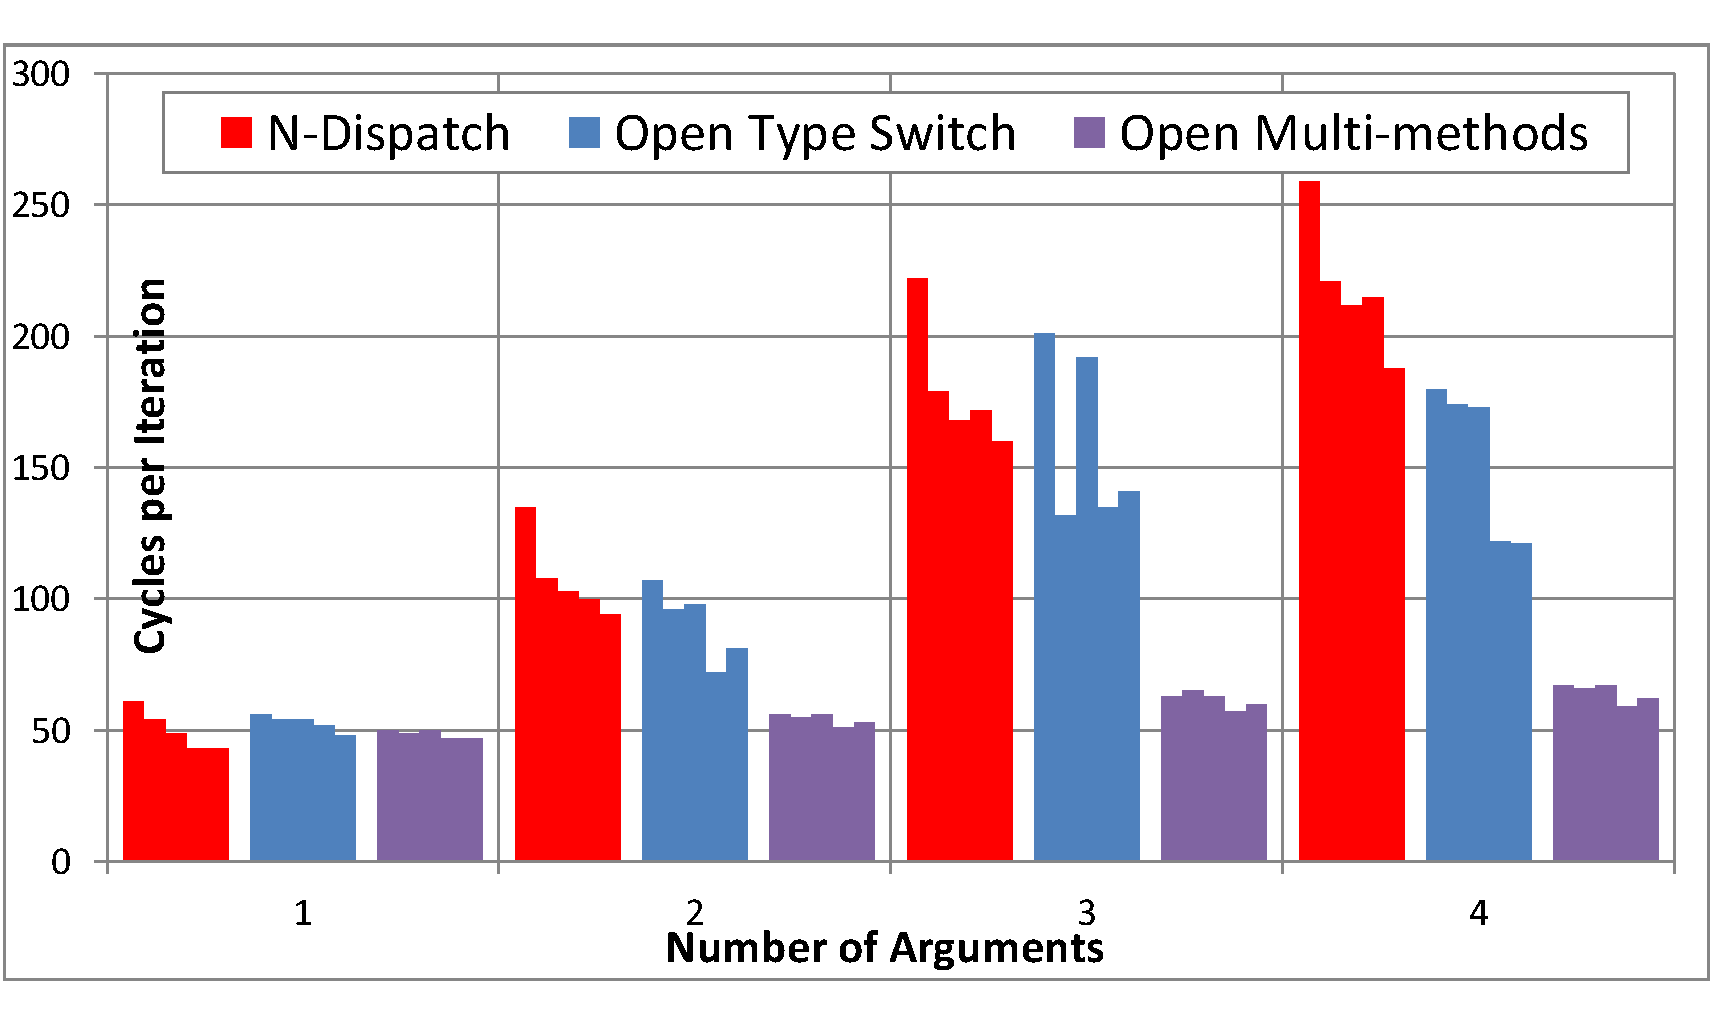
\includegraphics[width=0.49\textwidth]{Timing-N-arg.pdf}
  \caption{N-argument \code{Match}-statement vs. visitor design pattern and open multi-methods}
  \label{fig:dispatch}
\end{figure}

Open multi-methods provide the fastest performance because the dispatch is 
implemented with an $N$-dimensional array lookup, requiring only $4N+1$ memory 
references before an indirect call. N-Dispatch provides the slowest solution, 
requiring $2N$ virtual function calls (accept/visit per each dimension). Open 
type switch falls in between the two, thanks to its efficient hashing combined 
with a jump table.

In terms of memory, given a class hierarchy of $n$ classes (actually $n$ subobjects in 
the subobject graph) and a multiple dispatch on $N$ arguments 
from it, all 3 solutions will require the memory proportional to $O\of{n^N}$. 
More specifically, if $\delta$ is the number of bytes used by a pointer, then 
each of the approaches will use:

\begin{compactitem}
\setlength{\itemsep}{0pt}
\setlength{\parskip}{0pt}
\item Open Multi-Methods: $\delta\of{n^N+Nn+N}$
\item N-Dispatch: $\delta\of{n^N+n^{N-1}+\cdots+n^2+n}$
\item Open Type Switch: $\delta\of{\of{2N+3}n^N+N+7}$
\end{compactitem}

\noindent
bytes of memory. In all 3 cases the memory counted represents the non-reusable 
memory specific to the implementation of a single function dispatched through 
$N$ polymorphic arguments. Note that $n$ is a variable here since new classes 
may be loaded at run-time through dynamic linking in all 3 solutions, while $N$ 
is a constant, representing the number of arguments to dispatch on.

The memory used by each approach is allocated at different stages. The memory 
used by the virtual tables involved in the N-dispatch solution as well as 
dispatch tables used by open multi-methods will be allocated at compile/link 
time and will be reflected in the size of the final executable. Open 
multi-methods might require additional allocations and/or recomputation at load 
time to account for dynamic linking. In both cases, the memory allocated covers 
all possible combinations of $n$ classes in $N$ argument positions. In case of 
open type switch, the memory is only allocated at run-time and grows proportionally 
to the number of actual argument combinations seen by the type switch 
(\textsection\ref{sec:multiarg}). Only in the worst case when all possible 
combinations have been seen by the type switch does it reach the size described 
by the above formula. This is an important distinction as in many applications 
all-possible combinations will never be seen: for example, in a compiler the 
entities representing expressions and types might all be derived from a common 
base class, however they will rarely appear in the same type switch together.

There is also a significant difference in the ease of use of these solutions. 
N-Dispatch is the most restrictive solution as it is intrusive (and thus cannot 
be applied retroactively), hinders extensibility (by limiting the set of 
distinguishable cases) and is surprisingly hard to teach students. While 
analyzing Java idioms used to emulate multiple dispatch in practice, Muschevici 
et al~\cite[Figure 13]{MPTN08} noted that there are significantly more uses of 
cascading \code{instanceof} in the real code than the uses of double dispatch, 
which they also attribute to the obscurity of the second idiom. Both N-Dispatch 
and open multi-methods also introduce control inversion in which the case 
analysis is effectively structured in the form of callbacks. Open multi-methods 
are also subject to ambiguities, which have to be resolved at compile time and 
in some cases might require the addition of numerous overriders. Neither is the 
case with open type switch where the case analysis is performed directly, while 
ambiguities are avoided by the use of first-fit semantics.

%Although instanceof cascades may be slower than
%double dispatching, and are certainly less extensible, by
%being localised to a single class they are signi?cantly more
%straightforward to code than double dispatching. This may
%account for the relative popularity of each idiom.


\subsection{Rewriting Haskell code in \Cpp{}}
\label{sec:qualcmp}

For this experiment we took an existing code in Haskell and asked its author to 
rewrite it in \Cpp{} with \emph{Mach7}. The code in question is a simple 
peephole optimizer for an experimental GPU language called 
\emph{Versity}~\cite{Versity}. We assisted the author along the way to see which 
patterns he uses and what kind of mistakes he makes.

Somewhat surprising to us we found out that pattern-matching clauses generally 
became shorter, but their right-hand side became longer. The shortening of case 
clauses was perhaps specific to this application and mainly stemmed from the 
fact that Haskell does not support equivalence patterns or equivalence 
combinator and had to use guards to relate different arguments. This was 
particularly cumbersome when optimizer was looking at several arguments of 
several instructions in the stream, e.g.:

\begin{lstlisting}[language=Haskell]
peep2 (x1:x2:xs) = 
  case x1 of
    InstMove a b -> 
      case x2 of
        InstMove c d | (a == d) && (b == c) -> peep2 $ x1:xs
\end{lstlisting}

\noindent compared to \emph{Mach7} version:

\begin{lstlisting}
  Match(*x1,*x2) {
    Case(C<InstMove>(a,b), C<InstMove>(+b,+a)) ...
\end{lstlisting}

\noindent
Haskell also requires to use wildcard pattern in every unused position of a 
constructor pattern (e.g. \codehaskell{InstBin _ _ _ _}), while \emph{Mach7} 
allows one to omit all the trailing wildcards in constructor patterns (e.g. 
\code{C<InstBin>()}). And while this pays off only for constructor patterns with 
at least 3 arguments, the use of named patterns avoided many repeated pattern 
expressions and actually improved both performance and readability:

\begin{lstlisting}[columns=flexible]
  auto either = val(src) || val(dst);
  Match(inst) {
    Case(C<InstMove>(_,       either)) ...
    Case(C<InstUn>  (_, _,    either)) ...
    Case(C<InstBin> (_, _, _, either)) ...
  } EndMatch
\end{lstlisting}

\noindent
The disadvantage for \emph{Mach7} was coming after pattern matching, as we had to 
explicitly manage memory when inserting, removing or replacing instructions in 
the stream as well as explicitly manage the stream itself. Eventually we could 
hide some of this boilerplate behind smart pointers and other standard library 
classes.

During the initial rewrite into \Cpp{} the developer simply mapped Haskell 
patterns into their \emph{Mach7} equivalents, at which point we intervened and 
showed how some of the patterns can be expressed simpler. We reiterated the 
process until we could not improve the patterns ourselves without getting into 
the details of the actual simplifier. At one point we noticed that the developer 
started passing data via pattern-matching variables \code{var<T>} in and out of 
functions, which was not the intended use. This was hard to prevent statically, 
because in general, as first-class citizens, patterns can be passed in and out 
of functions, however in this case they were not used as patterns, but rather as 
values.

We have yet to make a performance comparison, but based on the performance of 
the open type switch~\cite{TS12} and the small overhead of our patterns, we 
expect the performance to be comparable.

\subsection{Limitations}
\label{sec:ommlimit}

While our patterns can be saved in variables and passed over to functions, they 
are not true first-class citizens. In fact, we believe that the notion of being 
a first-class citizen in a language should be updated to take parametric 
polymorphism of \Cpp{} into account. The reason is that as is, our solution does
not allow for composing patterns based on user's input (e.g. by letting user 
type in a pattern to match against). This can potentially be solved by mixing 
``patterns as objects'' approach in, however the performance overhead we saw in 
\textsection\ref{sec:patcmp} is too costly to be adopted.

\section{Related Work} %%%%%%%%%%%%%%%%%%%%%%%%%%%%%%%%%%%%%%%%%%%%%%%%%%%%%%%%%
\label{sec:rw}

Language support for pattern matching was first introduced for string 
manipulation in SNOBOL\cite{SNOBOL64}. SNOBOL4 had patterns as first-class data 
types providing operations of concatenation and alternation\cite{SNOBOL71}. The 
first reference to a modern pattern-matching constructs seen in functional 
languages is usually attributed to Burstall's work on structural 
induction\cite{Burstall69provingproperties}. Pattern matching was further 
developed by the functional programming community, most notably 
Hope\cite{BMS80}, ML\cite{ML90}, Miranda\cite{Miranda85} and 
Haskell\cite{Haskell98Book}. In the context of object-oriented programming, 
pattern matching has been first explored in Pizza\cite{Odersky97pizzainto} and 
Scala\cite{Scala2nd,EmirThesis}.

There are two main approaches to compiling pattern-matching code: the first is 
based on \emph{backtracking automata} and was introduced by Augustsson\cite{Augustsson85}, 
the second is based on \emph{decision trees} and was first described by 
Cardelli\cite{Cardelli84}, though he attributes the technique to Dave MacQueen 
and Gilles Kahn in their implementation of the Hope compiler \cite{BMS80}.
Backtracking approach usually generates smaller code, while decision tree 
approach produces faster code by ensuring that each primitive test is only 
performed once. With respect to matching a single expression our library 
approach follows the naive backtracking approach, however our match statement is 
based on a highly efficient type switching technique we developed\cite{TypeSwitch} 
that outperforms similar solutions based on decision trees or visitor design pattern.

Tom is a pattern-matching compiler that can be used together with Java, C or 
Eiffel to bring a common pattern matching and term rewriting syntax into the 
languages\cite{Moreau:2003}. It works as a preprocessor that transforms 
syntactic extensions into imperative code in the target language. Tom is quite 
transparent as to the concrete target language used and can potentially be 
extended to other target languages besides the three supported now.
Tom's  goals differ from ours in aiming to be a
tree-transformation language similar to Stratego/XT, XDuce and others. 
Tom's approach is prone to general problems of any preprocessor based 
solution\cite[\textsection 4.3]{SELL}. In particular, it is part of a dedicated toolchain.
Our library approach avoids that and lets us employ the C++ semantics within 
patterns: e.g. our patterns work directly on underlying user-defined data 
structures, avoiding abstraction penalties. The tight integration with 
the language semantics makes our patterns first-class citizens that can be 
composed and passed to other functions. 

Prop is another language extension that brings pattern matching into 
C++~\cite{Prop96}. This extension is not focused on pattern 
matching, but is intended for building high performance 
compiler and language transformation systems. It supports value-, variable-, 
wildcard-, constructor-, nested-, as-, type- and numerous sequence patterns.

Functional C\# is similar to our approach in trying to bring pattern matching 
into the C\# as a library\cite{FuncCSharp}. The approach uses lambda functions 
and chaining of method calls to create a structure that is then interpreted at 
run-time for the first successful predicate. The approach supports a form of 
active patterns, simple n+k patterns, list and tuple patterns as well as type 
patterns (without structural decomposition). 
However, an approach based on sequential type tests 
scales very poorly for match statements with more than two case clauses, making 
it unreasonably slower than the visitor design pattern~\cite{TypeSwitch}. Besides, the approach 
seems to be ill suited for tests involving nesting of patterns.

When the class hierarchy is fixed, one can design a pattern language that involves 
semantic notions represented by the hierarchy. Pirkelbauer devised a pattern 
language for Pivot capable of representing various entities in a C++ program using syntax very close to the C++ itself. 
Interestingly, the patterns were translated with a tool into a set of visitors 
implementing the underlying pattern-matching semantics\cite{PirkelbauerThesis}. 
Earlier, Cook et al used expression templates to implement a query language for 
Pivot's class hierarchy~\cite{iql04}. Our current work is the result of a series 
of experimental designs. The library approach was essential to provide 
relatively quick turnaround for experiments and for maintaining and improving 
performance for our applications.

\section{Conclusions and Future Work} %%%%%%%%%%%%%%%%%%%%%%%%%%%%%%%%%%%%%%%%%%
\label{sec:cc}

We present a pattern-matching library for \Cpp{} that provides fairly standard
pattern-matching facilities. Our solution is non-intrusive and can be 
retroactively applied. %to any polymorphic or tagged  
%class hierarchy. It also provides a uniform notation to these different 
%encodings of algebraic and extensible hierarchical data types in \Cpp{}.
The library provides efficient and expressive matching on multiple subjects and 
compares to multiple dispatch alternatives in terms of both time and space.

We generalize n+k patterns to arbitrary expressions by letting the user define 
the exact semantics of such patterns. Our approach is more general than traditional approaches 
as it does not require an
equational view of such patterns. It also avoids hardcoding the 
exact semantics of n+k patterns into the language. 

We used the library to rewrite existing code that relied heavily on the 
visitor design pattern.
Our pattern matching code was much shorter (both source and object code), 
simpler, easier to maintain, comprehend, and faster. 
This confirmed our view of the visitor pattern as a clever workaround,
rather than a good solution to a fundamental problem.
The library approach was essential 
for experimentation in the context of real programs and for delivering 
performance comparable with or superior to conventional techniques in the 
context of industrial compilers.

The work presented here continues our research on pattern matching for 
\Cpp{}~\cite{TS12}. We plan to further experiment with other kinds of patterns, 
including those defined by the user, look at the interaction of patterns with 
other facilities in the language and the standard library, and make views less 
ad hoc. For example, standard containers in \Cpp{} do not have the implicit 
recursive structure present in data types of functional languages, and viewing 
them as such with views would incur significant overheads. We will experiment 
with very general patterns as first-class citizens.

Our generalization of n+k patterns depends on the properties of types involved 
in the expression. This should let us experiment not only with generic 
functions, but also with their generic inversions in the form of solvers. As 
more \Cpp{}11 features become available in compilers it will also be interesting to 
look at how use of these features affects the ease of use, performance, 
readability, writability and debugging of the library and the user code that 
uses it.

%In the nearest future, we would like to make our library to be safe and efficient 
%in a multi-threaded environment. 

%From Morten Rhiger:
%New languages are often constructed by piling new features on top of an existing language's de?nition and by integrating these features in the existing language's implementation. However, it is a sign of expressiveness if new features can be implemented within an
%existing language without changing its de?nition.
%Short of macros, functional languages such as Haskell and Standard ML require new
%features to be expressed in terms of typed higher-order functions. We have demonstrated
%how to extend - or, in Guy Steele's terminology, to "grow" (Steele Jr., 1999) - Haskell
%with our own statically typed implementation of pattern matching and we have shown how
%to extend this framework with patterns not currently supported by Haskell.


\balance
\bibliographystyle{abbrv}
%\bibliographystyle{abbrvnat}
\bibliography{mlpatmat}

%\appendix
%\section{\Cpp{} Concepts} %%%%%%%%%%%%%%%%%%%%%%%%%%%%%%%%%%%%%%%%%%%%%%%%%%%%%%
\label{sec:prelim}

TODO: Describe everything we use from concepts:

\begin{itemize}
\item concept definition
\item refinement of another concept
\item associated functions
\item associated types
\item associated templates (we have those, e.g. accepted\_type\_for)
\item default implementation of an associated function
\item requires
\item concept-based overloading
\item decltype
\item std::declval
\item template aliases
\end{itemize}

The following concepts can be used as examples since we later refer to them in 
the paper: \code{CopyConstructible}, \code{Convertible}.

Concepts were not included in \Cpp{}11, so we emulate them using overloading and 
\code{enable_if}~\cite{jarvi:03:cuj_arbitrary_overloading}.

\end{document}
